%%%%%%%%%%%%%%%%%%%%%%%%%%%%%%%%%%%%%%%%%%%%%%%%%%%%%%%%%%%%%%%%%%%%%%%%
%                                                                      %
% LaTeX, FIIW thesis template                                          %
% 28/11/2014 v1.2                                                      %
%                                                                      %
%%%%%%%%%%%%%%%%%%%%%%%%%%%%%%%%%%%%%%%%%%%%%%%%%%%%%%%%%%%%%%%%%%%%%%%%
\documentclass[11pt,a4paper]{report}
% Indien je je thesis recto-verso wil afdrukken gebruik je onderstaande opties i.p.v. bovenstaande
%\documentclass[11pt,a4paper,twoside,openright]{report}

\usepackage[a4paper,left=3.5cm, right=2.5cm, top=3.5cm, bottom=3.5cm]{geometry}
\usepackage[dutch]{babel}
\usepackage{graphicx}
\usepackage[latin1]{inputenc}           % om niet ascii karakters rechtstreeks te kunnen inputten
%\usepackage[utf8]{inputenc}            % commentarieer deze regel uit als je utf8 encoded files gebruikt in plaats van latin1
\usepackage{natbib}
\usepackage{listings}             		% voor het weergeven van broncode
\usepackage{verbatim}					% weergeven van code, commando's, ...
\usepackage{hyperref}					% maak PDF van de thesis navigeerbaar
\usepackage{url}						% URL's invoegen in tekst met behulp van \url{http://}
\usepackage[small,bf,hang]{caption}     % om de captions wat te verbeteren
\usepackage[final]{pdfpages}            % gebruikt voor het invoegen van het artikel in pdf-formaat
\usepackage{pslatex}					% andere lettertype's dan de standaard types

\usepackage{sectsty}					% aanpassen van de fonts van sections en chapters
\allsectionsfont{\sffamily}
\chapterfont{\raggedleft\sffamily}

\usepackage{float}                      % De optie H voor de plaatsing van figuren op de plaats waar je ze invoegt. bvb. \begin{figure}[H]
%\usepackage{longtable}					% tabellen die over meerdere pagina's gespreid worden
%\usepackage[times]{quotchap}           % indien je fancy hoofdstuktitels wil
%\usepackage[none]{hyphenat}
%\usepackage{latexsym}
%\usepackage{amsmath}
%\usepackage{amssymb}
\usepackage{amsmath}
\usepackage{fiiw_denayer}
% \usepackage{fiiw_denayer_eng} % For the english version (also change last page at the bottom of this file!

%door onderstaande regels in commentaar te zetten, of op false, kan je pagina's weglaten
%bijvoorbeeld het weglaten van een voorwoord, lijst met symbolen, ...
%%%%%%%%%%%%%%%%%%%%%%%%%%%%%%%%%%%%%%%%%%%%%%%%%%%%%%%%%%%%%%%%%%%%%%%%%%%%%%%%%%%%%%%%
%voorwoord toevoegen?
\acknowledgementspagetrue
\acknowledgements{voorwoord}			%.tex file met daarin het voorwoord
%abstract toevoegen?
\abstractpagetrue
\abstracts{abstract}					%.tex file met daarin het abstract

%lijst van figuren toevoegen?
\listoffigurespagetrue
%lijst van tabellen toevoegen?
%\listoftablespagetrue
%lijst van symbolen toevoegen?
%\listofsymbolspagetrue
%\listofsymbols{symbolen}				%.tex file met daarin de lijst van symbolen



%informatie over het eindwerk, de promotor, ...
%%%%%%%%%%%%%%%%%%%%%%%%%%%%%%%%%%%%%%%%%%%%%%%
\opleiding{Elektronica - ICT}
\afdeling{ICT}

\title{Automatische detectie van pati\"entengedrag in hun slaapomgeving}
\subtitle{ }
% \author{naam student}
\forename{Nele}
\surname{Annaert}
\academicyear{2016 - 2017}

\promotorA[Promotor(en)]{Prof. Dr. Ir Toon Goedem\'e}
\promotorB[Co-promotor(en)]{Ir Jasmien Vanvooren}

\begin{document}
\selectlanguage{dutch}
% \selectlanguage{english} % For the english version
\preface

%Het eerste hoofdstuk van je thesis.
\chapter{Inleiding}
Deze masterproef behandelt een onderzoek naar het gebruik van camera beveiliging in een slaapomgeving. Met als doel te detecteren wanneer een persoon uit bed stapt en langs welke zijde dit gebeurt. Is het mogelijk om dit te doen? Welke camera kunnen we het best gebruiken? Dit zijn de vragen waar de vooral een antwoord op willen geven. \\
We zijn begonnen met het kijken naar welke verschillende systemen er al zijn en welke technieken interessant kunnen zijn voor ons. We bespreken zo verschillende generaties van surveillance systemen, verschillende types van camera en verschillende methoden om personen te detecteren. Vooral op voorgond achtergrond segmentatie wordt dieper ingegaan. \\
Vervolgens bespereken we een paar experimenten die we gedaan hebben. Onze experimenten zijn in verschillende stappen gebeurd. We beginnen zeer eenvoudig met het opslaan en ophalen van afbeeldingen. Vervolgens gaan we verder met de effectieve persoon detectie. Nadat de persoon gedetecteerd wordt, gaan we verder met de detecte van de zijde waarlangs er uit bed gestapt wordt. Om dit te kunnen bereiken maken we gebruik van temporeel verschil. Als allerlaatste hebben we ons algoritme toegepast op live beelden. \\
Uit de kleine experimenten hebben we elk keer onze belsuiten getrokken en nieuwe experimenten uitgevoerd. Dit tot we uiteindelijk aan het algemeen besluit komen. 

\chapter{Literatuurstudie}
In dit hoofdstuk gaan we nakijken of er reeds werken geschreven zijn die voor ons toepasselijk zijn. Voor we beginnen aan het maken van het project, gaan we eerst op zoek naar reeds bestaande systemen, deze worden beschreven in sectie \ref{refRBS}, we bekijken welke types van surveillance systemen er bestaan en bestuderen welke eventueel interessant kunnen zijn voor ons project in sectie \ref{refTVS}, dit wordt gevolgd door sectie \ref{refTVC}, deze omvat  een beschrijving van verschillende types van camera's. Als laatste deel van de literatuurstudie bestuderen we reeds bestaande algoritmes voor persoonsherkenning in sectie \ref{refAVPH}. Dit hoofdstuk wordt afgesloten in sectie \ref{refLBe} met een besluit over de literatuurstudie.

\section{Reeds bestaande systemen}
\label{refRBS}
Het eerste wat we onderzochten was of er al gelijkaardige systemen bestonden. Onze zoekacties op het internet leverden aanvankelijk geen resultaten op. Al blijkt dat er in bijvoorbeeld de slaapkliniek van A.Z. Monica ook gewerkt word met een infraroodcamera. Daarover was verder geen informatie te vinden. Gedurende de rest van het jaar bleven we verder zoeken naar soort gelijke systemen, omdat de mogelijkheid altijd bestaat dat er nieuwe informatie beschikbaar komt.

\section{Types van surveillance systemen}
\label{refTVS}
In dit deel van de literatuurstudie gaan we onderzoeken welke types van surveillance systemen er zijn. We gaan eveneens bestuderen welke types zinvol zijn voor ons project. Waarom zouden we werken met camerabeveiliging? Je zou ook een systeem kunnen maken door gebruik te maken van druk sensoren in een mat naast het bed, of onder de matras zelf. Het voordeel van camera gestuurde surveillance is dat we kunnen zien wat er op het moment zelf gebeurt, maar dat we ook achteraf gebeurde incidenten kunnen reconstrueren. Het nadeel van camera gestuurde surveillance is dat we incidenten moeten kunnen identificeren en herkennen op het  moment dat ze gebeuren \cite{bibVTC3}. Er zijn drie verschillende generaties van surveillance systemen. De eerste generatie van surveillance systeem dat we gaan bestuderen is het traditionele surveillance systeem, meer informatie hierover is terug te vinden in sectie \ref{refTST}, daarna gaan we verder met de tweede generatie van surveillance systemen in sectie \ref{refTGS}, dit wordt gevolgd in sectie \ref{refINS} door een bespreking van de intelligente surveillance systemen.  Een surveillance systeem kan door middel van verschillende parameters ge\"evalueerd worden. Bijvoorbeeld door een studie van de tijdsvertraging tussen het voorvallen van een gebeurtenis en de detectie. Er wordt momenteel ook nog steeds onderzoek gedaan op gebied van de verschillende types van camera gestuurde surveillance.

\subsection{Traditionele surveillance systemen}
\label{refTST}
De traditionele surveillance systemen zijn de eerste van drie generaties van surveillance systemen. Ze maken gebruik van analoge technologie doorheen het volledige systeem, dit is een van de grootste nadelen van dit type van systeem \cite{bibIPC2}.  Analoge camera's maken in dit type van systeem, de beelden van de sc\`ene. De signalen worden verzonden over communicatielijnen naar de  toestellen, waar de data weergegeven en opgeslagen worden \cite{bibVTC2}. In een traditioneel surveillance systeem is de kwaliteit en de kost recht evenredig met het aantal gebruikte camera's. Voor een grote omgeving, worden er voor een systeem meerdere camera's gebruikt, om een hele omgeving te bestuderen. Bijgevolg wordt er een grote hoeveelheid aan data verzameld die achteraf verwerkt moet worden.  In onze toepassing, moet er enkel het bed bestudeerd worden. Hierdoor hebben wij een kleine omgeving en volstaat het om \'e\'e camera te hebben voor de detectie van het patienten gedrag. Indien er ook valdetectie gedaan wordt, zijn er  twee camera's nodig om een dieptebeeld te cre\"eren. Meestal is er een persoon nodig die altijd naar de monitor kijkt \cite{bibVTC}. Omdat wij meerdere pati\"enten in het oog willen houden, is dit voor ons niet mogelijk. In sommige gevallen geeft deze methode zeer goede resultaten.

\subsection{Tweede generatie surveillance systemen}
\label{refTGS}
In de tweede generatie van surveillance systemen wordt er gebruik gemaakt van digitale componenten. De overstap van analoge naar digitale technologie is nog niet compleet. Er wordt een combinatie van beide technologie\"en. Automatische visuele surveillance wordt hier mogelijk door een combinatie van computer visuele technologie met Closed Circuit Television (CCTV) systemen \cite{bibIPC2}. Hierdoor is de detectie van gebeurtenissen eenvoudiger voor de gebruiker. Deze dient eens het programma geschreven is en de detecties automatisch doet, zelf niets meer te doen. De alarmtijd wordt korter. Doordat een computer de detectie doet, en niet meer een persoon, kunnen we elke kamer uitrusten met een surveillance systeem. Bij traditionele surveillance systemen zou dit gelijk zijn als voor elke kamer een persoon te betalen om de kamers te bewaken. Door de automatisatie kunnen  we meerdere kamers in het oog gehouden worden. De kwaliteit van het surveillance systeem is beter \cite{bibVTC2}, dit doordat de reactie tijd hoger is. E\'en van de nadelen is dat je algoritmes nodig hebt voor de gedragsanalyses \cite{bibIPC2}. Het ontwikkelen van deze gedragsanalyses gaat tijden de ontwikkel fase veel tijd in beslag nemen. Eens deze ontwikkelt zijn en goede resultaten hebben, gaan zij bijdragen tot de betere resultaten van het surveillance systeem ten opzichte van de traditionele systemen. Het ontwikkelen van dergelijk gedragsanalyse omvat het grootste deel van het onderzoek dat in dit werk gedaan wordt. 

\subsection{Intelligente surveillance}
\label{refINS}
Dit is het derde en eveneens laatst generatie van beeld gestuurde surveillance systemen. Hier is de overgang naar een volledig digitaal systeem compleet\cite{bibVTC2}. Daarom wordt het vaak een intelligent surveillance systeem genoemd. Het kan automatisch zeer grote regio's verwerken. Een groot voordeel is dat er verschillende soorten van sensoren kunnen gecombineerd worden waardoor er zeer veel informatie beschikbaar is. Het opzetten van een dergelijk systeem is moeilijker dan het opzetten bij de voorgaande generaties. men moet het systeem trainen om de incidenten te detecteren. Men  kan dit zowel manueel als computergestuurd doen. Hoe meer data je nodig hebt om het systeem te trainen, hoe meer men het proces moet automatiseren \cite{bibVTS}. Het verwerken van de beelden die gemaakt worden gebeurt in verschillende stappen.  Welke stappen deze zijn en in welke volgorde ze gebeuren, zijn te zien in figuur \ref{imgVTS} \cite{bibIPC2}.
\begin{figure}[hbp]
	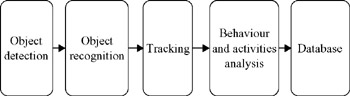
\includegraphics[scale=0.8]{FlowSurveillance}
	\caption{Traditionele flow voor het verwerken van beelden in een surveillance systeem}
	\label{imgVTS}
\end{figure}

\section{Verschillende types van camera's}
\label{refTVC}
In het tweede deel van de literatuurstudie doen we onderzoek naar verschillende types van camera's. En bekijken of deze al dan niet bruikbaar zijn voor ons project. Waarom zijn niet alle camera's geschikt? Aangezien het project gaat over het bestuderen van het slaapgedrag van pati\"enten, gaan onze beelden gemaakt worden in een donkere omgeving. Hierdoor zal er met sommige camera's bijna niets te zien zijn. Het eerste type van camera dat we bespreken is de infraroodcamera in sectie \ref{refIRC}, dit type camera werkt met warmte-verschillen. Een ander type van camera dat we mogelijk ook kunnen gebruiken is  de night vision camera, deze wordt besproken in sectie \ref{refNVC}. Dit is een type van camera speciaal ontworpen om in donkere omgevingen te werken. Een derde mogelijk type van camera wordt besproken in sectie \ref{refIPZ}, namelijk een IP-camera. Nadat we de werking van de IP camera bekijken, gaan we deze uitbereiden met PTZ-camera's, dit is terug te vinden in sectie \ref{refIPC2}.

\subsection{Infraroodcamera}
\label{refIRC}
We hebben het vermoeden dat de infrarood (IR) camera interessant kan zijn omdat deze warmte-verschillen weergeeft. In tegenstelling tot camera's die opereren in de zichtbare band van het spectrum werkt de IR camera  een lange golflengte (8-12 $\mu$m). Een IR sensor gaat de elektromagnetische golven, die zich in het spectrum van de  camera bevinden, uitgestraald door objecten in een sc\`ene, als een thermische afbeelding weergeven,. Waarvan elke pixelwaarde een temperatuur voorstelt \cite{bibIRC2}. We gaan dus de persoon, indien deze zich binnen het bereik van de camera bevindt waarnemen, ongeacht of het dag of nacht is. Dit komt doordat de temperatuur van een pati\"ent, normaal gezien, hoger is als deze van de omgeving \cite{bibIRC3}.
De eerste bedenkingen hierbij zijn of het mogelijk is om een persoon te detecteren als deze gebruik maakt van een elektrisch warmtedeken. Verder gaat het bed ook opwarmen. We moeten dus ook bekijken of er geen valse persoonsdetecties gebeuren op de warme lakens als de persoon in kwestie niet meer in het bed ligt. Verder is de camera ongevoelig voor lichtinval. Hierdoor gaat het bijvoorbeeld geen schaduwen maar ook geen kleuren van kleding waarnemen. Een voordeel van dit type camera is dat een persoon al onherkenbaar is op de beelden. Dit is \'e\'en van de vereisten van ons systeem. Een probleem doet zich voor wanneer een pati\"ent naar de badkamer gaat en er vervolgens een ander persoon de kamer binnen komt. Dit  zal in de beelden zeer weinig verschil veroorzaken en er kunnen valse detecties gebeuren.  Een ander probleem dat opduikt is dat er kringen verschijnen rond gebieden met een zeer hoge of zeer lage temperatuur \cite{bibIRC4}. De sterkte en grootte van deze kringen is afhankelijk van het actuele temperatuurverschil tussen de persoon en de omgeving, en de contrast/gain instellingen van de camera \cite{bibBET6}. Een van de grote voordelen is de uitzonderlijk lage signal to noise ratio (SNR). In het begin werd de IR camera voornamelijk in militaire toepassingen gebruikt. Door de daling van de prijs van een infrarood camera wordt deze tegenwoordig steeds vaker gebruikt in verschillende toepassingen zoals bijvoorbeeld industri\"ele inspectie, door de politie en ook in surveillance systemen\cite{bibBET6}. Op het internet zijn er ook veel verschillende manieren te vinden om van een oud fototoestel zelf een infraroodcamera te maken. Al blijken deze niet altijd goed te werken.
Dankzij de vele toepassingen en de dalende prijs, zijn er ook veel bedrijven die met IR camera's op de markt komen die door ons gebruikt kunnen worden. Hieronder is een lijst te vinden met een paar voorbeelden van dergelijke bedrijven.
\begin{itemize}
	\item Heimann Sensor
	\item Excelitas met CoolEye sensor
	\item Panasonic in samenwerking met AS electronic
	\item Infinitegra
	\item Seek Thermal
\end{itemize}

\subsection{Night vision camera}
\label{refNVC}
\begin{figure}[hbp]
	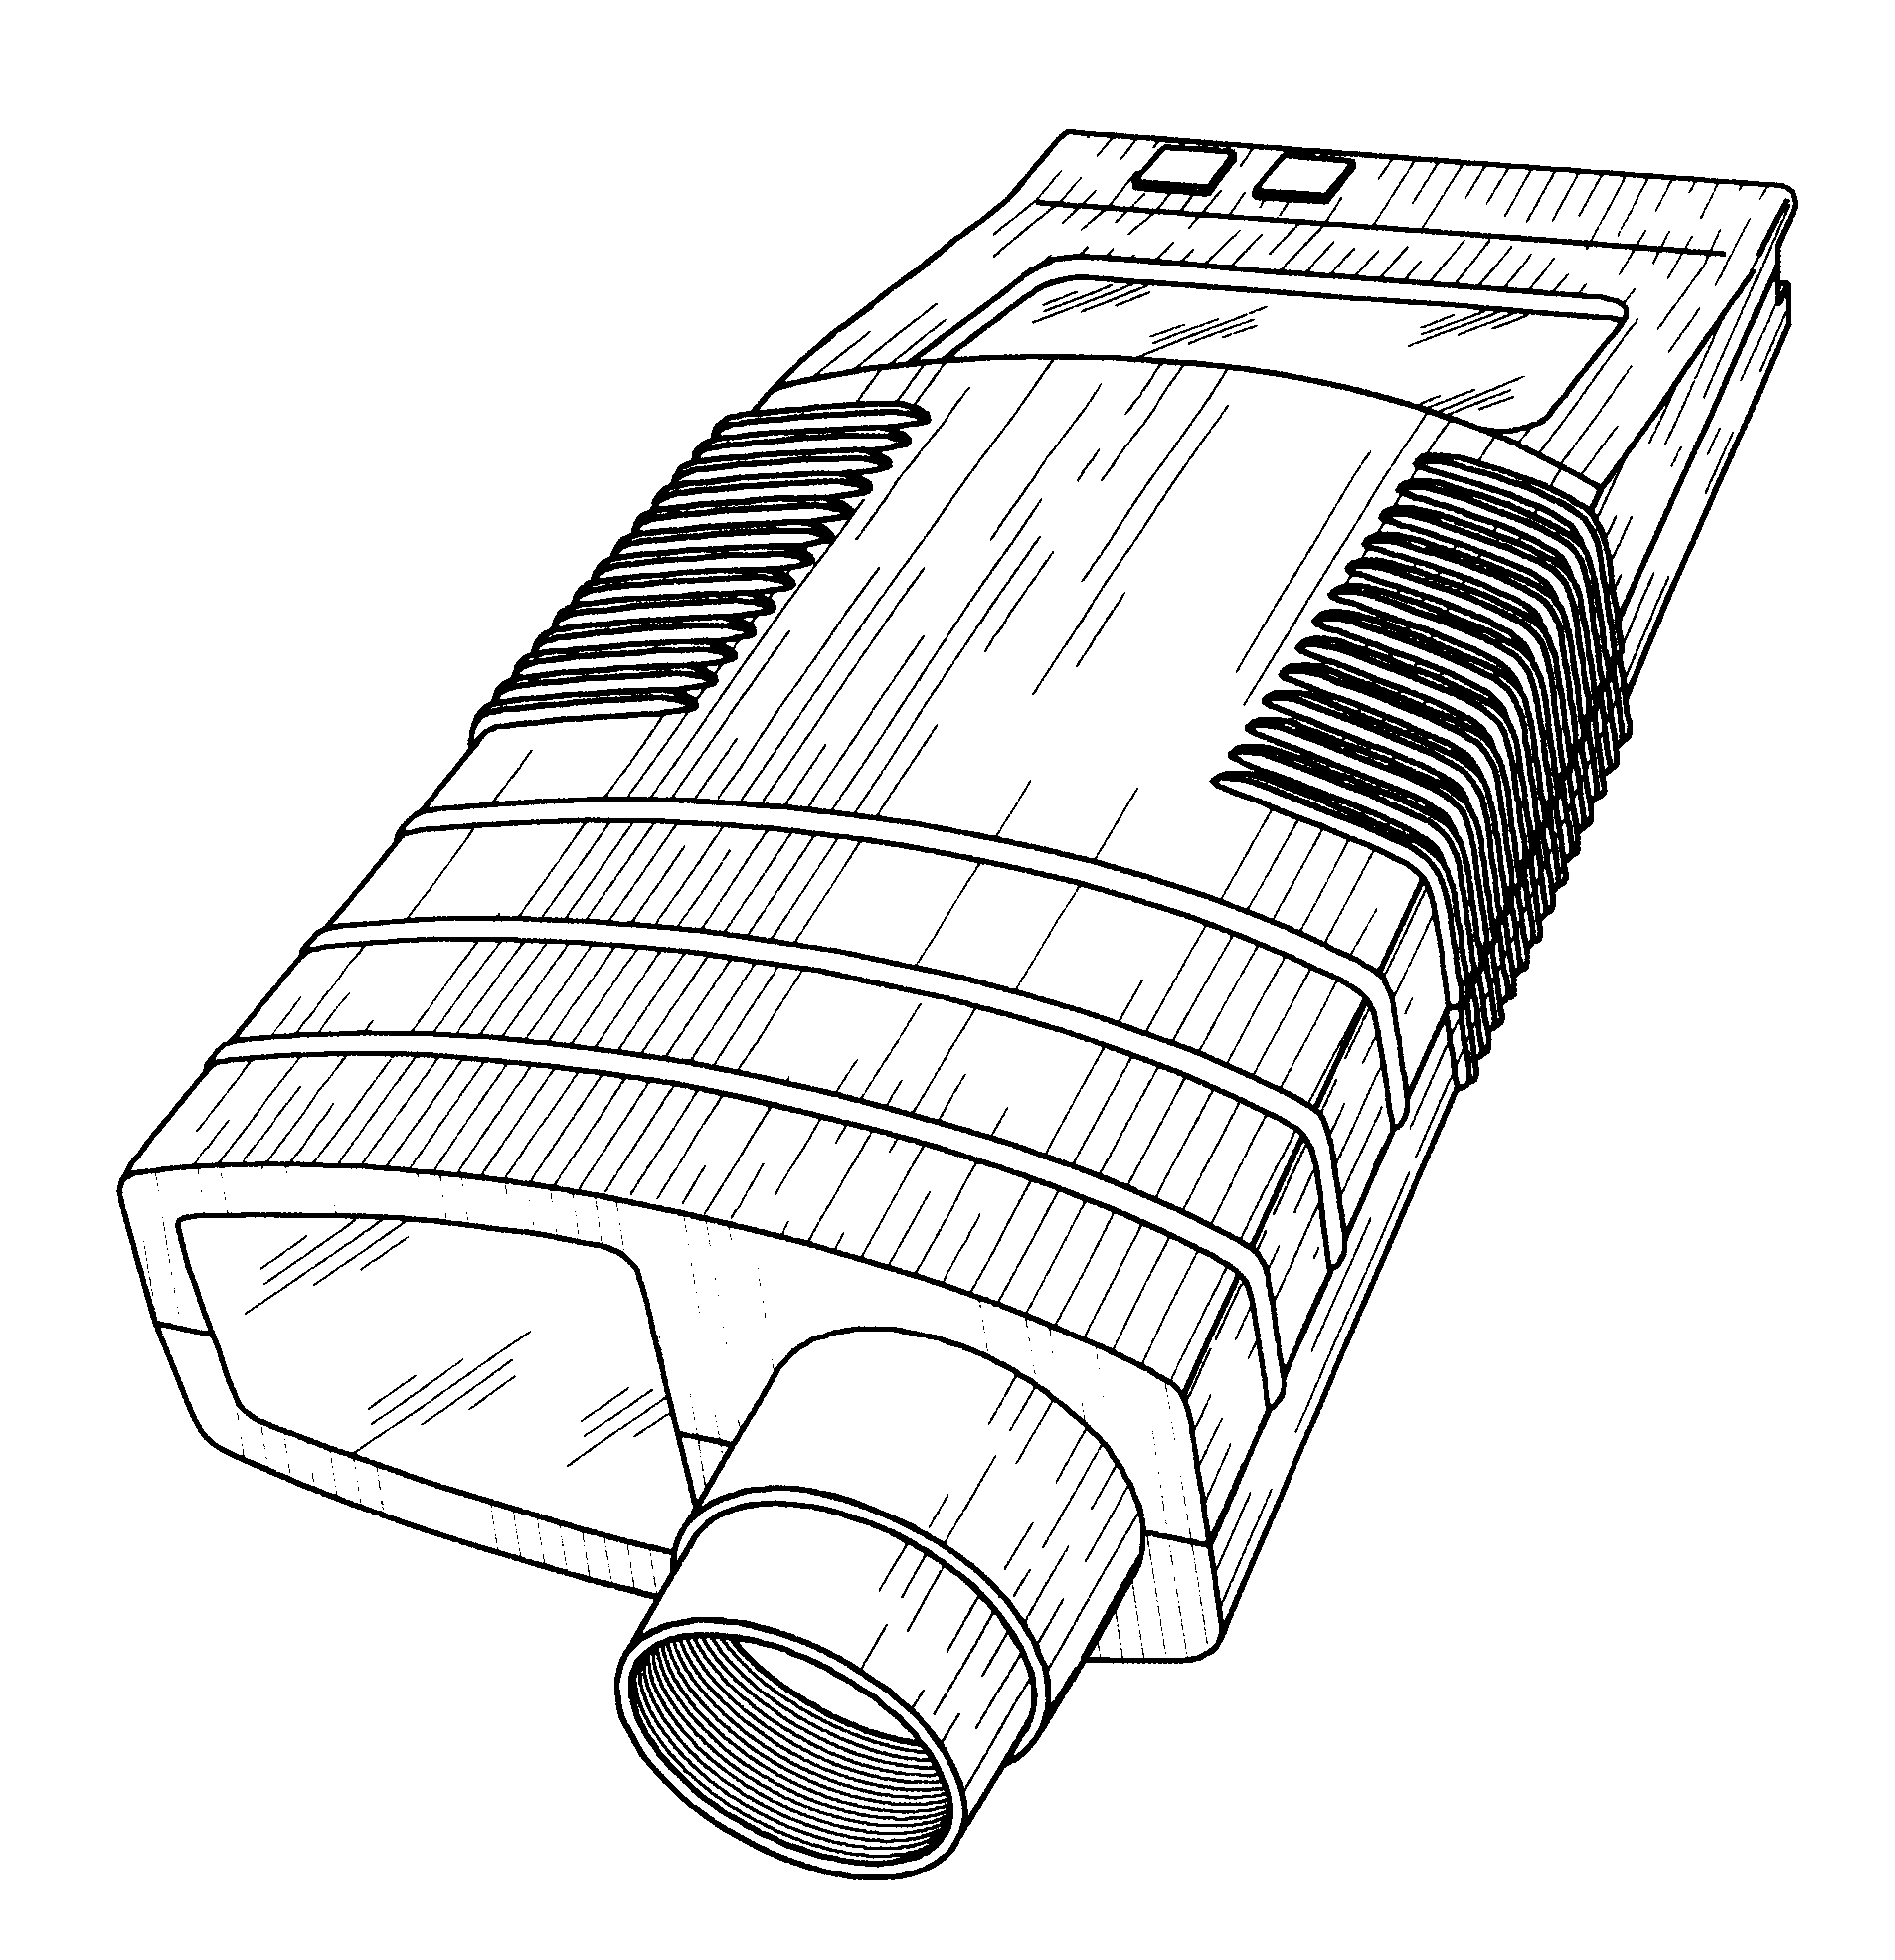
\includegraphics[scale=0.075]{NightVisionCamera}
	\caption{Afbeelding van een night vision camera}
	\label{imgNVC}
\end{figure}
Een ander type van camera dat ook mogelijkheden biedt, is een night vision camera. Een afbeelding van zo een camera, is te vinden in figuur \ref{imgNVC}\cite{bibNVC}.
Dit type van camera wordt gebruikt in een omgeving waar onvoldoende licht is voor een standaardcamera en wordt voornamelijk bij zonsondergang, 's nachts of zonsopgang gebruikt. Dit type van camera wordt in veel toepassingen gebruikt waaronder surveillance, astronomie en gedragsonderzoek van dieren \cite{bibNVC2}. Aangezien wij 's nachts onze beelden maken en deze zouden gebruikten voor een surveillance systeem, vallen wij in het gebruiksgebied van deze camera. Er wordt gebruik gemaakt van SWIR dit is kleine golflengte infrarood, met een golflengte van (1-1.7 $\mu$m). Deze SWIR gaat het overgebleven atmosferisch licht, dat 5 tot 7 keer groter is dan het licht van de sterren, waarnemen. Het maken van de beelden in SWIR gebeurt op een vergelijkbare manier dan in een standaardcamera, het is het resultaat van een reflectie principe . De dure versies gaan beelden gemaakt met LWIR (Lange golflengte IR) combineren met SWIR beelden \cite{bibNVC2}. Het nadeel van deze camera is dat de persoon wel herkenbaar is op de beelden die rechtstreeks komen van de camera. Terwijl in de vereisten van ons systeem staat dat de persoon onherkenbaar moet zijn op de beelden. Dit kan natuurlijk achteraf door middel van beeldverwerking aangepast worden, door bijvoorbeeld een masker te cre\"eren door huidsegmentatie toe te passen op de beelden. Deze camera's zijn duurder dan de eerder besproken IR camera's in sectie \ref{refIRC}.

\subsection{IP camera}
\label{refIPC}
IP staat voor Internet Protocol. Het is een camera voorzien van de mogelijkheid om verbinding te maken met het internet. De camera functioneert op je computer netwerk. De camera wordt aangesloten aan een router, switch of draadloos netwerk.  De camera combineert de traditionele camera en netwerk video technologie. De IP camera kan live video comprimeren in de camera zelf wordt de video data omgezet naar digitale data, die al voor een deel verwerkt is. Enkel een abstracte beschrijving van het beeld wordt verder gestuurd \cite{bibIPC3}.  De data wordt over het internet verzonden zonder daarvoor een computer te gebruiken. De basis architectuur van de IP camera ziet u in figuur \ref{imgIPC} \cite{bibVTC2}.
\begin{figure}[hbp]
	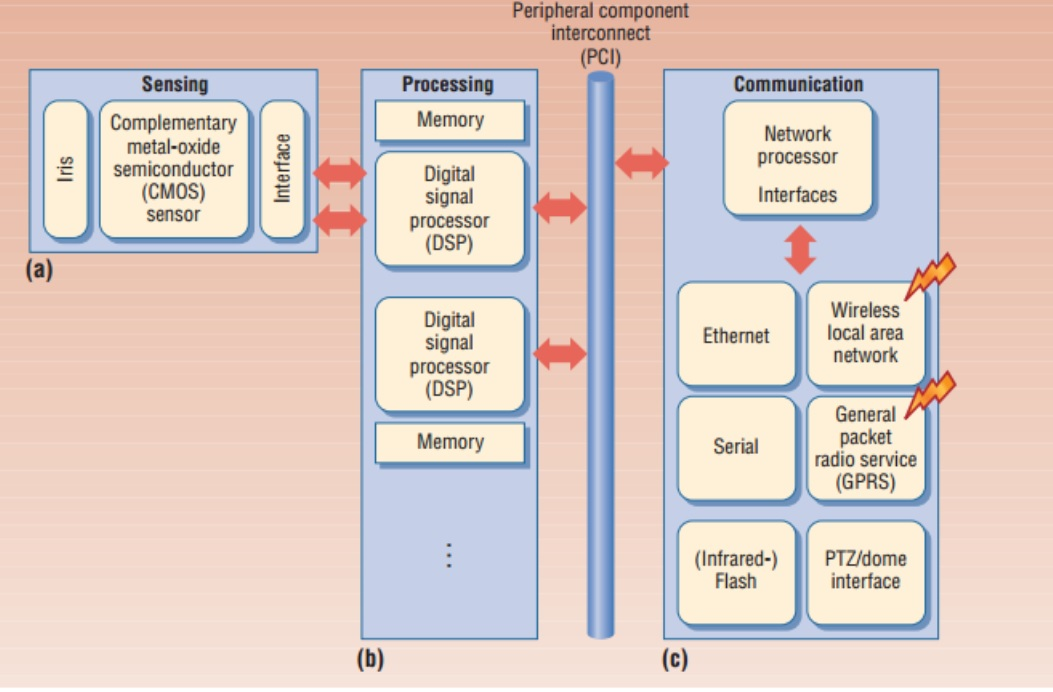
\includegraphics[scale=0.55]{ArchitectuurIPCamera}
	\caption{Hardware architectuur IP camera bestaande uit 3 delen: (a) Sensor eenheid, (b) Verwerkings eenheid, (c) Communicatie eenheid.}
	\label{imgIPC}
\end{figure}
De camera is opgebouwd uit drie delen. Het eerste deel is de sensor eenheid, deze bestaat meestal uit een zeer dynamische monochrome complimentary metal-oxide semiconductor (CMOS) afbeelding sensor. In sommige gevallen komen hier ook andere sensoren bij. Het tweede deel van de architectuur, is de afhandelingseenheid. Deze bestaat uit Digital Signal Processor (DSP). Zij bieden een goede compromis tussen prestatie, vermogen verbruik en flexibiliteit.  De verbinding met de netwerk processor wordt tot stand gebracht door Perpiheral Component Interconnect (PCI) bus. De netwerk processor gaat zorgen voor de interconnectie tussen de communicatie- en afhandelingseenheden. Indien er nog verdere afhandeling van de beelden nodig is, zijn er een paar vaste stappen: object detectie en herkenning, volgen, gedragsanalyse en ophalen van de data \cite{bibIPC2}. Er zijn verschillende soorten van IP camera's, je hebt er voor gebruikt binnen en buiten, of speciaal uitgerust voor gebruik 's nachts, al dan niet met infrarood. De camera die wij nodig hebben is er \'e\'en voor binnen, die uitgerust is voor 's nachts. Het prijskaartje hiervan kan al snel oplopen tot een paar honderden euro's. Dit type camera wordt vooral gebruikt voor bewakingssystemen, ook in de medische sector, verder vormen ze ook de kern van surveillance in de toekomst.

\subsection{IP en PTZ camera's}
\label{refIPC2}
De uitbereiding van twee IP camera's met een PTZ camera wordt gedaan, om een dieptebeeld te kunnen vormen. Dit is nodig voor een mogelijke uitbereiding van dit onderzoek, namelijk de detectie van een pati\"ent die uit bed valt.  We beginnen met twee IP camera's om de positie en locatie van een persoon te bepalen, deze worden automatisch uit de beelden van de camera's gehaald. De positie en locatie worden dan doorgestuurd naar een Pan-Tilt-Zoom (PTZ) camera. De camera wijst en zoomt naar de juiste locatie in de ruimte. In ons geval dus naar de pati\"ent. Hierdoor wordt van de persoon een goed kwalitatief beeld gevormd. Het ontwerp van zo een systeem is te zien in figuur \ref{imgIPC2} \cite{bibIPC}. De grootste moeilijkheid bij dergelijke constructie is dat je de goniometrische relatie tussen de verschillende camera's moet kennen. Om ervoor te zorgen dat dit in orde is kan je een kalibratie doen. Het is door deze goniometrische relatie dat de co\"ordinaten bepaald worden waar de PTZ camera's op gaan inzoomen. \cite{bibVTC3}. Een groot nadeel van deze opstelling is natuurlijk de extra kost van een IP camera en een PTZ camera. We moeten ook de afweging maken of het verkrijgen van een nauwkeuriger beeld van de pati\"ent door de PTZ camera het maken van de extra kost waard is. Anders zouden wij ook de opstelling zonder PTZ camera kunnen gebruiken om de diepte te kunnen bepalen voor de valdetectie.
\begin{figure}[hbp]
	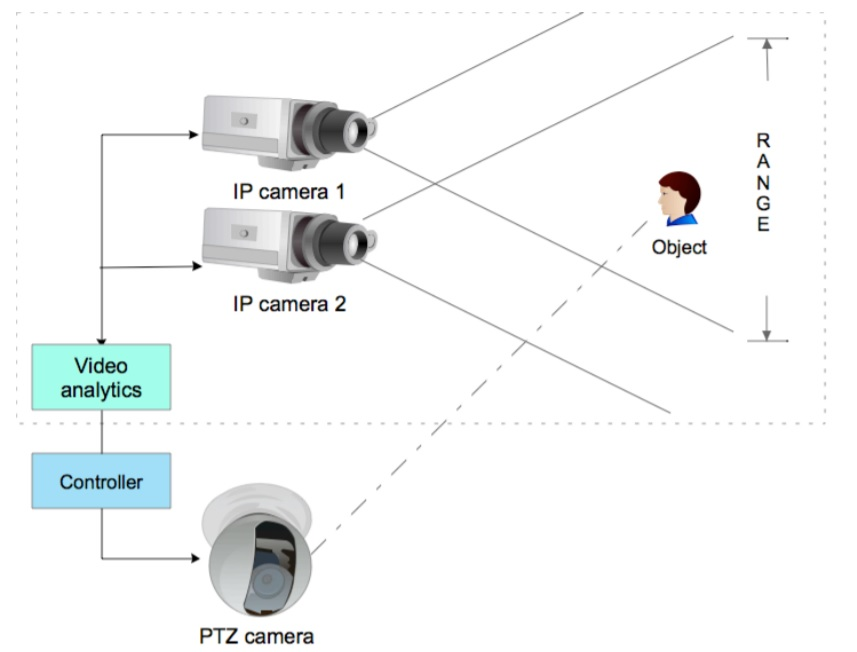
\includegraphics[scale=0.5]{IPPTZCamera}
	\caption{Systeem ontwerp met twee IP camera's en een PTZ camera}
	\label{imgIPC2}
\end{figure}

\section{Algoritmes voor persoonsherkenning}
\label{refAVPH}
In dit hoofdstuk bespreken we algoritmes voor persoonsherkenning. Deze hebben we nodig om de pati\"ent uit het frame te halen. Er zijn veel verschillende methodes ontwikkeld. In dit hoofdstuk bespreken we er een paar die we onderzocht hebben.  De eerste techniek is het thresholden van kleuren, alle informatie hierover is te vinden in sectie \ref{refTVK}. Hierna wordt background estimation techniek of voorgrond- achtergrondsegmentatie besproken in sectie \ref{refBET}. Deze techniek vaak gebruikt voor het volgen van mensen en bewegingen. Ze zijn vooral bruikbaar bij een stationaire camera \cite{bibIRC}. Aangezien wij in ons onderzoek een stationaire camera hebben, is dit voor ons een zeer interessante techniek. Een nadeel is dat elke vorm van verandering wordt gedetecteerd als de pati\"ent, waardoor het soms kan lijken dat er meerdere pati\"enten in een kamer zijn en er dus valse detecties kunnen optreden. Een oplossing hiervoor is een vorm gebaseerde benadering, die we zullen bespreken in sectie \ref{refVBB} \cite{bibIRC}. In de meeste gevallen worden verschillende van deze methoden gecombineerd op uiteindelijk goede resultaten te krijgen. 

\subsection{Thresholden van kleuren}
\label{refTVK}
Dit algoritme is gebaseerd op de kleuren dat een object heeft op de beelden. Deze techniek kan voor veel applicaties gebruikt worden, zoals het detecteren van personen, zoals ook onze bedoeling is, of bijvoorbeeld het detecteren van het rood uit verkeersborden. Deze methode is pixel gebaseerd, voor elke pixel wordt de kleurwaarde vergeleken met een regio in het kleurenspectrum. Zo kunnen we in onze toepassing pixel per pixel zien of het al dan niet gaat om een persoon \cite{bibTHK}. Er zijn verschillende systemen om kleuren te benoemen, bijvoorbeeld:
\begin{description}
	\item[RGB] Rood Groen en Blauw
	\item [CMY] Cyaan, Magentha and Yellow: De primaire kleuren van de kleurpigmenten
	\item [HSI] Hue, Saturation and Intensity
	\item [YUV] Y = helderheid en UV chrominantie (kleurcomponenten)
\end{description}
We kunnen in het algoritme spelen met de verschillende systemen, zo kunnen we zien waar de persoon het makkelijkst uit het beeld te halen is. Indien we dit algoritme gebruiken, gaan we gebruik maken van OpenCV. Om de ruis achteraf te gaan verminderen, kunnen we erosie en dillatie, een median filter of een andere methode gebruiken. 
 
\subsubsection{Jones and Rehg}
Ze maakten een model op basis van internet afbeeldingen. Ze onderzochten welke kleuren in welke verhoudingen voorkomen in de huidskleur op de verschillende afbeeldingen. Nadat dit model af was hebben ze een ander model toegevoegd dat huid- en niet huidafbeeldingen scheidt. Ze maakten een huidhistogram waarin ze de kleur verhoudingen van huid gelabelde afbeeldingen staken, ze maakten ook een niet-huidhistogram waarin ze de kleur verhoudingen van niet-huid gelabelde afbeeldingen staken. Dankzij deze histogrammen kan men de kans berekenen dat huid voorkomt in een bepaalde pixel \cite{bibTHK}. Doordat wij onze beelden 's nachts maken en er dan weinig lichtinval is, gaan in onze toepassing, de kleurwaarden anders zijn. Verder gaan wij ook op beelden gemaakt met een infraroodcamera geen huidskleur zien. Bijgevolg is dit dus een techniek die niet van toepassing is voor ons onderzoek. 

\subsubsection{Dawod et al.}
Dit model staat ook gekend als het RGB-H-CbCr model. Dit is een pixel gebaseerde methode. De beelden worden bekeken in drie verschillende kleurruimtes. De eerste kleurruimte is het RGB domein. Vervolgens wordt gebruik gemaakt van het HSV-domein en als laatste het YUV-domein. Een andere naamgeving voor het YUV domein is H-Cb-Cr. Hierbij geeft H de waarde van de gereflecteerde luminantie. Cb staat voor chrominantie blauw en geeft het verschil aan tussen een referentiewaarde en de blauwe component. Cr is chrominantie rood en geeft het verschil weer tussen een referentiewaarde en de rode component. Deze kleurruimte wordt typisch gebruikt voor huiddetectie \cite{bibDEA}. In elke kleurruimte wordt er beslist of een pixel al dan niet huid is. Achteraf worden de drie ruimtes samengevoegd en besloten of een pixel al dan niet huid is, de huidpixels moeten een aaneensluitende regio vormen \cite{bibTHK}. Doordat we onze beelden 's nachts maken gaan de waarden van de kleuren veranderd zijn. Hierdoor kunnen we ook deze techniek niet gebruiken voor onze toepassing.

\subsection{Voorgrond- achtergrond segmentatie}
\label{refBET}
Deze techniek wordt ook background estimatation genoemd. De techniek is gebaseerd op het feit dat een beeld bestaat uit een achtergrond die niet verandert en een voorgrond die dus alle bewegende en veranderde delen bevat. Eens de achtergrond bepaald is, wordt deze van het nieuwe frame afgetrokken. De verschilwaarde wordt dan vergeleken met een drempelwaarde. Als de verschilwaarde groter is dan de drempelwaarde, wordt ze op de resultaten afbeelding op 1 gezet, indien ze kleiner is dan de  drempelwaarde wordt die pixel op de resultaten afbeelding 0. Ze krijgt men een binair beeld. Dit is terug te vinden in figuur \ref{imgVAS} \cite{bibVAS}.

\begin{figure}[hbp]
	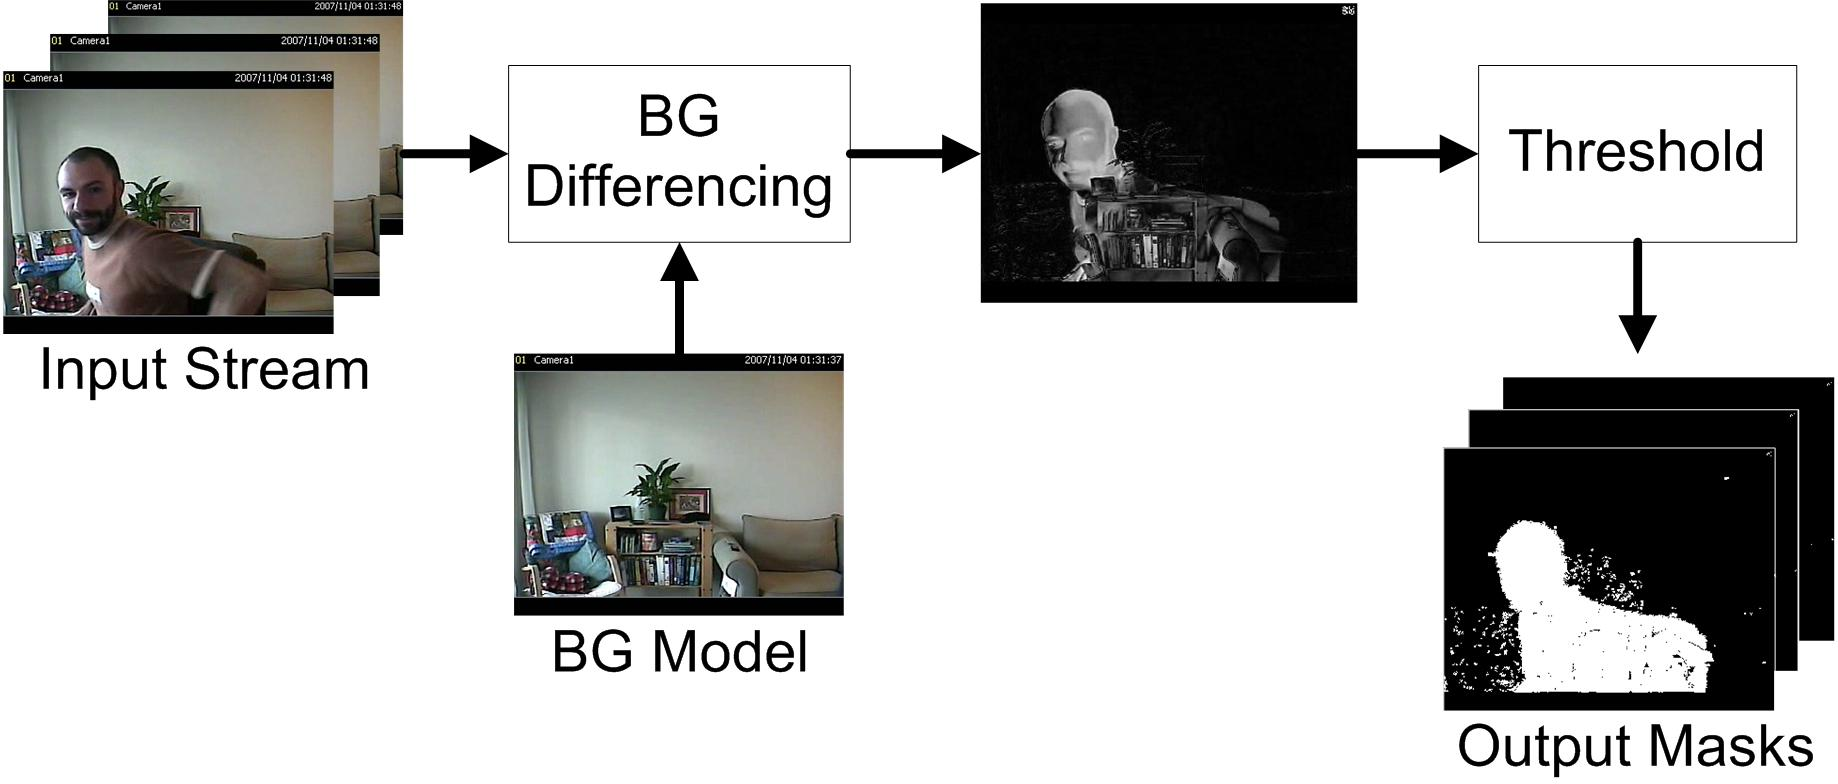
\includegraphics[scale=0.65]{BackgroundSegmentation}
	\caption{Voorbeeld voorgrond/achtergrond segmentatie}
	\label{imgVAS}
\end{figure}

Voorgrond- achtergrond segmentatie wordt vaak gebruikt in video surveillance \cite{bibBET3}. Deze techniek kan je splitsen in twee verschillende types namelijk recursief en niet-recursief. Eerst bespreken we de recursieve technieken. Dit wordt gevolgd door de niet-recursieve technieken. Elk van deze technieken kan op verschillende manieren gebeuren en heeft zijn voordelen en nadelen op vlak van geheugen, snelheid en moeilijkheid. De eerste stap van de deze techniek is het bepalen van de achtergrond. Dit kan op drie verschillende manieren gebeuren, namelijk per pixel per regio en per frame \cite{bibBET4}.  Dit gebeurt in de achtergrondmodelleringsfase. De voorgrond- achtergrond segmentatie techniek heeft 2 verschillende nadelen. Het eerste nadeel is dat hij licht gevoelig is, als je het licht aan doet, verandert het beeld. Hierdoor kunnen in bepaalde toepassingen valse detecties optreden  \cite{bibBET4}. Het tweede nadeel is dat de techniek gevoelig is voor de beweging van de camera. Je kan deze techniek dus enkel toepassen op beelden gefilmd met een statische camera \cite{bibBET7} of door de beweging in het algoritme te reduceren. Een derde nadeel is dat het niet mogelijk is om goede resultaten te bekomen bij een niet statische achtergrond of in geval van ruis \cite{bibBET9}. Als allerlaatste bespreken we een manier om voorgrond/achtergrond segmentatie toe te passen op thermische beelden \cite{bibBET5},\cite{bibBEt},\cite{bibBET2}. Vaak worden verschillende technieken gecombineerd om betere resultaten te krijgen.\\
Voorgrond/achtergrond segmentatie technieken moeten met 3 zaken rekening houden om succesvol te zijn \cite{bibBET8}:
\begin{itemize}
	\item Wat is het model en hoe gedraagt het zich?
	\item Hoe wordt het model ge\"initialiseerd?
	\item Hoe wordt het model ge\"updatet?
\end{itemize}
Doordat in onze toepassing de camera en de achtergrond statisch is. En de beelden 's nachts gemaakt worden, waardoor er weinig invloed is van het licht. Zijn de drie grote nadelen van deze methode hier niet van toepassing. Hierdoor kunnen we mogelijk \'e\'en van de verschillende soorten voorgrond- achtergrond segmentatie gebruiken in onze toepassing.
 
\subsubsection{Recursieve technieken}
\label{refRT}
Het achtergrond model wordt op recursieve wijze bij elke frame ge\"updatet. Dit wordt eveneens een adaptieve techniek genoemd. Omdat de achtergrond die bij het eerste frame geschat wordt, bij elke frame aangepast wordt, totdat de achtergrond bijna niet meer wijzigt. Het voordeel hiervan is dat je geen extra frames moet bewaren in een buffer. Het nadeel hiervan is dat als er zich een fout voordoet in het achtergrond model dit ook voor lange tijd in het achtergrond model bewaard blijft. We bespreken vier verschillende recursieve methodes om de achtergrond te bepalen. De eerste techniek is running avarage,  de tweede is de approximated median filtering gevolgd door mixture of gaussian en om af te sluiten bespreken we $\Sigma$ - $\Delta$ achtergrond segmentatie.

\paragraph{Running avarage}
\label{refRUA}
Het achtergrond model wordt voor deze techniek bepaald aan de hand van volgende formule \cite{bibBEt}:
\begin{displaymath}
A_{i+1}=\alpha F_i+(1-\alpha)A_i
\end{displaymath}
met:
\begin{description}
	\item[A\textsubscript{i}] De nieuwe achtergrond die bepaald wordt
	\item[A\textsubscript{i}] De huidige achtergrond
	\item[$\alpha$] De leersnelheid, vaak 0.05, met een waarde tussen 0 en 1
	\item[F\textsubscript{i}] De huidige frame
\end{description}
Dit wilt zeggen dat het achtergrond model gemaakt wordt door voor elke pixel de gemiddelde waarde te nemen van de waarde in de vorige achtergrondschatting en de huidige framewaarde. De achtergrond gaat dus mee veranderen in de loop van de tijd. \\
Men kan de voorgaande formule generaliseren door het te schijven in incrementele vorm \cite{bibSDB}:
\begin{displaymath}
A_{i+1}=A_i+\delta_t F_i
\end{displaymath}
met:
\begin{description}
	\item[A\textsubscript{i}] De nieuwe achtergrond die bepaald wordt	
	\item[A\textsubscript{i}] De huidige achtergrond
	\item[$\delta_t$] increment functie, afhankelijk van de huidige frame
	\item[F\textsubscript{i}] De huidige frame
\end{description}
De voordelen van deze methode zijn
\begin{itemize}
	\item Eenvoudige berekeningen die niet veel CPU tijd vragen
	\item Er wordt niet veel geheugen gevraagd
	\item De bepaling van de achtergrond gaat heel snel in verhouding tot andere technieken
	\item De methode is eenvoudig te implementeren.
	\item Houdt rekening met veranderingen in de achtergrond
\end{itemize}
De nadelen van deze methode zijn
\begin{itemize}
	\item Het resultaat is een schatting en is dus niet precies
	\item $\alpha$ moet geregeld worden om zo nauwkeurig mogelijke resultaten te krijgen.
	\item De nauwkeurigheid van de achtergrond-schatting is afhankelijk van de snelheid waarmee het object door het beeld beweegt.
\end{itemize}
Er is ook een niet recursieve tegenhanger, deze noemt men exponential smoothing \cite{bibSDB}. Doordat een persoon tijdens het slapen niet veel beweegt, gaat op de plaats waar de persoon slaapt, de persoon als achtergrond gelabeld worden. Als de persoon vervolgens beweegt, gaat er een geest, een persoon die er niet is, ontstaan op de slaapplaats. Wij gaan op dat moment twee personen detecteren terwijl er maar \'e\'en is. Als we gebruik maken van deze techniek, moeten we in het algoritme met deze geest rekening houden en zien dat we de re\"ele persoon gebruiken.

\paragraph{Approximated Median Filtering}
\label{refAMF}
Deze methode heeft ook een niet recursieve tegenhanger. Omdat ze zo'n goede resultaten opleveren en de berekening zeer eenvoudig is. Het principe is als volgt: als de grijswaarde van de pixel die men bekijkt groter is dan de grijswaarde van de geschatte achtergrond, wordt de grijswaarde van deze pixel in de geschatte achtergrond ge\"incrementeerd met 1. Dezelfde redenatie voert men ook uit als de grijswaarde van de pixel kleiner is dan de grijswaarde van de overeenkomstige pixel in de geschatte achtergrond. De waarden van de achtergrond gaan convergeren naar de effectieve mediaan \cite{bibVTS}.Deze techniek werkt omdat men ervan uit gaat dat de achtergrondpixels gedurende het grootste deel van de tijd zichtbaar zijn. Daardoor is de effectieve mediaan de achtergrond. Dit resulteert in weinig rekenwerk.\\
De voordelen van deze methode zijn:
\begin{itemize}
	\item Zeer eenvoudige implementatie
	\item Hoge nauwkeurigheid
	\item Niet veel geheugen nodig
	\item De techniek is robuust
\end{itemize} 
De nadelen van deze techniek zijn:
\begin{itemize}
	\item Als er een wijziging is in de achtergrond, past hij zich maar traag aan
\end{itemize}
Deze techniek heeft hetzelfde nadeel als de voorgaande, de persoon word tijdens het slapen als achtergrond aangeduid. Als de persoon dan gaat bewegen wordt er een geest gecre\"eert. Het achtergrond model gaat zich wel aanpassen en de geest zal verdwijnen, maar het gaat lang duren.

\paragraph{Mixture of Gausian}
\label{refMOG}
Mixture of gausian ook wel MOG genoemd, zal aan de hand van een model bepalen of een pixel tot de voor- of achtergond hoort. Als de waarde van de pixel in het huidige frame hoort binnen de waarden van de achtergrond, zal deze tot de achtergrond gerekend worden. Het updaten van de achtergrond is afhankelijk van de waarschijnlijkheid van de waarden van het nieuwe frame. De waarden waarmee ge\"incrementeerd worden zijn eveneens afhankelijk van de dichtheid van de achtergrond. Als de dichtheid groter is, zal de incrementeer waarde ook groter zijn \cite{bibSDB}. Het aantal Gausische distributies die gebruikt worden tijdens de berekening, weergegeven door k, is afhankelijk van de hoeveelheid beschikbaar geheugen. \\
De formule is hieronder te vinden \cite{bibMOG}:
\begin{displaymath}
	P(X_{t}) = \sum_{i=1}^{k} w_{i,t} * \eta (X_{t},\mu_{i,t},\sum{i,t})
\end{displaymath}
met:
\begin{description}
	\item[k] Het aantal Gausische distributies	
	\item[w\textsubscript{i,t}] een schatting van het gewicht van de i\textsuperscript{de} Gaussian op ogenblik t
	\item[$\mu$\textsubscript{i,t}] de gemiddelde waarde van de i\textsuperscript{de} Gaussian op ogenblik t
	\item[$\sum{i,t}$] De covariantie matrix van de i\textsuperscript{de} Gausian op ogenblik t
	\item[$\eta$] Gausische probaliteits functie
	\item[X\textsubscript{t}] De pixelwaarde op het ogenblik t
\end{description}
De formule van de Gausische probaliteitsfunctie, is hieronder weergegeven \cite{bibMOG}:
\begin{displaymath}
\eta (X_{t},\mu_{i,t},\sum{i,t}) = \frac{1}{(2\pi)^{\frac{n}{2}}|\sum|^{\frac{1}{2}}}e^{-\frac{1}{2}(X_t-\mu_t)^T\sum^{-1}(X_t-\mu_t)}
	\end{displaymath}
	met:
	\begin{description}
		\item[X\textsubscript{t}] De pixelwaarde op het ogenblik t
		\item[$\mu$\textsubscript{i,t}] de gemiddelde waarde van de i\textsuperscript{de} Gaussian op ogenblik t
		\item[$\sum$] De covariantie matrix van de i\textsuperscript{de} Gausian op ogenblik t
		\item[T] Schatting van de minimale hoeveelheid data dat tot de achtergrond gerekend wordt
	\end{description}
Voordelen van de methode:
\begin{itemize}
	\item Er is geen vaste drempelwaarde
	\item Deze methode is nauwkeuriger dan de running avarage en approximated median filtering methodes die eerder beschreven werden.
	\item Kan tegen lange termijn veranderingen en herhalende bewegingen.
\end{itemize}
Nadelen van deze methode:
\begin{itemize}
	\item Deze methode is traag.
	\item Veel moeilijke berekeningen nodig om de achtergrond te bepalen
\end{itemize}
De nadelen wegen zwaarder op dan de voordelen. Daardoor wordt deze techniek minder vaak gebruikt \cite{bibSDB}, \cite{bibMOG}.

\paragraph{ $\Sigma$ - $\Delta$ achtergrond segmentatie}
De $\Sigma$ - $\Delta$ achtergrond segmentatie is een eenvoudige, niet lineaire methode om de achtergrond te bepalen \cite{bibSDB}. Het wordt vaak gebruikt in ingebedde toepassingen \cite{bibBET8}. Om de achtergrond te bepalen wordt aangenomen dat de achtergrond voor het grootste deel van de tijd zichtbaar is \cite{bibSDB2}. Het is gebaseerd op vergelijken en elementaire optellingen en verschillen. 
Door middel van een functie bepaalt men de waarschijnlijkheid van de waarde van de pixel van de volgende frame, dit noemt men het dichtheidsmodel .  Hoe hoger de waarschijnlijkheid van een pixel, hoe kleiner de nood om het te gaan updaten, hierdoor is de geschatte achtergrond stabieler. \cite{bibSDB2} Men gaat dan de pixelwaarde vergelijken met de waarde van het dichtheidsmodel en de waarde van de achtergrond aanpassen. Een mogelijke manier om de geschatte waarde te bepalen is door gebruik te maken van de Zipf law, dit is een hyperbolisch afnemende functie. Ook hier treedt het apperture probleem op, dit wilt zeggen dat de middelste delen van bewegende delen niet mee gedetecteerd worden. De relevantie van deze techniek is te vergelijken met die van MOG \cite{bibSDB}.\\
Voordelen van de methode:
\begin{itemize}
	\item Eenvoudig te berekenen
\end{itemize}


\subsubsection{Niet recursieve technieken}
\label{refNRT}
De niet-recursieve technieken maken gebruik van een sliding window benadering voor het bepalen van de achtergrond. De laatste frames worden opgeslagen in de buffer en de achtergrond wordt bepaald door temporele variatie van elke pixel. Het voordeel van deze methode is dat ook personen die lang in dezelfde houding op het bed liggen ook gedetecteerd worden. Het nadeel hiervan is dat de buffer een groot deel geheugen in beslag neemt. Er zijn verschillende methodes om het achtergrond model te bepalen. We bespreken er drie, als eerste bespreken we temporeel verschil, de tweede methode is temporeel verschil met drie frames, als laatste bespreken we median filter.

\paragraph{Temporeel verschil}
\label{refFRD}
Dit is een zeer eenvoudige model. Deze methode wordt gebruikt om bewegende objecten uit een reeks van afbeeldingen te halen. De gedetecteerde oppervlakken omvatten de doel oppervlakken en kleine oninteressante oppervlakken (bijvoorbeeld kleine veranderingen in de achtergrond) \cite{bibTeV}. Je neemt twee opeenvolgende frames, neemt daarna het verschil, dit verschil wordt dan vergeleken met een drempelwaarde. \cite{bibIPC2}. Aangezien een pati\"ent in zijn slaap heel weinig gaat bewegen, is dit voor ons geen goede methode. Hoe weet anders het systeem of de persoon stil in bed ligt of hij uit het beeld verdwenen is? Een nadeel van deze techniek is dat men gebruik maakt van een sequentie van beelden en dat de detectie dus een paar frames later gebeurt. \cite{bibIRC}. De techniek kan zeer goed tegen dynamische veranderingen van de omgeving. Maar geeft niet alle relevante pixels als oplossing, er ontstaan gaten in bewegende objecten. \cite{bibTVD}.
\begin{displaymath}
|frame_{i}-frame_{i-1}|>T
\end{displaymath}
met
\begin{description}
	\item [frame\textsubscript{i}] het huidige frame
	\item [frame\textsubscript{i-1}] het vorige frame
	\item [T] de drempelwaarde
\end{description}
Als het verschil groter is dan de drempelwaarde, dan hoort die pixel bij de voorgrond. \cite{bibBET3}. De drempelwaarde wordt empirisch bepaald.\\
Voordelen:
\begin{itemize}
	\item Weinig rekenkracht nodig.
	\item De methode is zeer adaptief.
	\item Er wordt zeer weinig extra geheugen gebruikt.
	\item Het model wordt snel bijgewerkt als er iets verandert in de achtergrond.
\end{itemize}
Nadelen:
\begin{itemize}
	\item Als een persoon niet beweegt, verdwijnt deze mee in de achtergrond.
	\item Als een object een gelijkmatig verdeelde intensiteit waarden heeft, de middelste delen mee verdwijnen in de achtergrond
	\item Deze methode is zeer gevoelig voor ruis.
	\item Het is moeilijk om de juiste drempelwaarde te vinden.
	\item Een kleine verandering in de achtergrond wordt mee als voorgrond gezien 
\end{itemize}
\cite{bibTeV}

\paragraph{Temporeel verschil met drie frames}
Deze methode is een uitbereiding op de methode die we in de vorige paragraaf hebben besproken. Het grootste verschil is dat er drie opeenvolgende frames gebruikt worden om de achtergrond te berekenen. Het blok diagram van deze methode vindt u in figuur \ref{imgTeV}. 
Zoals u in de figuur kan zien, zijn er verschillende stappen in het algoritme. Hieronder gaan we ze stap voor stap uitleggen.
\begin{figure}[h]
	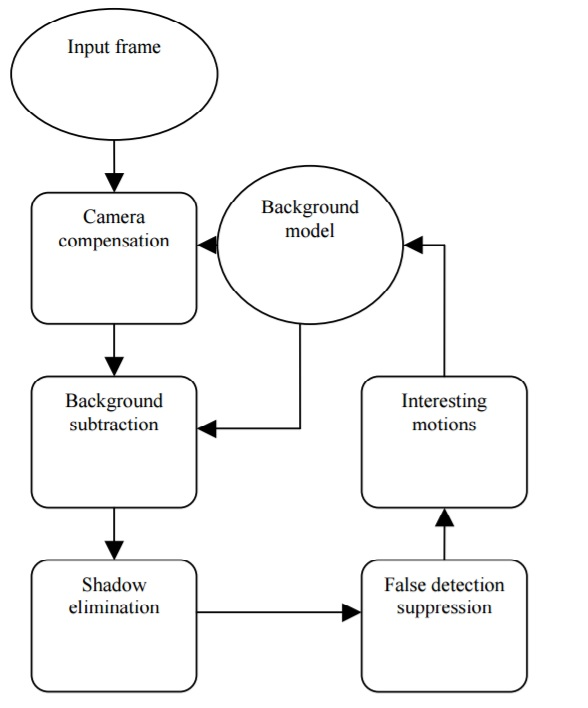
\includegraphics[scale=0.6]{TemporeelVerschilDrieFrames}
	\caption{Blokschema temporeel verschil van drie Frames}
	\label{imgTeV}
\end{figure}

\subparagraph{Camera compensatie}
Hier worden eventuele kleine bewegingen van de camera gecompenseerd, omdat temporeel verschil heel gevoelig is aan kleine veranderingen in het beeld. Dit gebeurt door middel van een algoritme dat enkele standaard pixels in het frame neemt en vervolgens de beweging schat door middel van een matching methode. Vervolgens wordt het volledige inputframe aangepast.  Indien je werkt met een statische camera hoef je deze stap niet te doen.

\subparagraph{Temporeel verschil door middel van drie frames}
Vervolgens wordt het temporeel verschil gebruikt om snel de bewegende objecten uit het input beeld te halen. De drie frames worden verdeeld in twee groepen. De eerste groep bevat de twee voorgaande frames, de tweede groep bevat de input frame en het voorgaande frame. Van deze twee groepen wordt dan het temporeel verschil zoals besproken in de voorgaande paragraaf berekend. Vervolgens kan men door de intersectie te nemen van de twee berekende verschillen eenvoudig de beweging berekenen van het vorige frame, deze komt namelijk in de twee berekeningen voor. Vervolgens neemt men het verschil van het temporeel verschil van de tweede groep en de juist berekende intersectie. Nu houd je de bewegende delen over van het laatste frame.

\subparagraph{Overige stappen}
De stappen na de berekening van het temporeel verschil worden gebruikt om de twee problemen die optreden door het gebruikt van de methode ongedaan te maken. De eerste is dat het onmogelijk is om altijd het volledig bewegende object te detecteren, dit doordat er kleine gaten ontstaan in het bewegend object door de berekening van het temporeel verschil. Het tweede is dat deze techniek heel gevoelig is voor kleine veranderingen en er dus ook oninteressante regio's zijn die gedetecteerd worden \cite{bibTeV}.

\paragraph{Median Filter}
\label{refMEF}
Deze techniek wordt zeer vaak toegepast. Hij zegt dat de mediaan van elke pixel van de n laatste  frames in de buffer de achtergrond is. De redenatie hierachter is dat de achtergrond in de helft van de frames ongewijzigd gaat blijven.\\
Voordelen:
\begin{itemize}
	\item Weinig rekenkracht voor nodig.
	\item Levert vrij nauwkeurige resultaten.
\end{itemize}
De nadelen van deze methode zijn
\begin{itemize}
	\item Vrij veel geheugen capaciteit nodig.
\end{itemize}


\subsubsection{Per pixel proces}
\label{refPPP}
Men kijkt naar elk pixel signaal als een onafhankelijk proces. Deze methode wordt tegenwoordig het meeste gebruikt omdat men hiervoor weinig rekenkundige kracht nodig heeft. Al de methodes die hierboven besproken werden zijn per pixel processen. Het principe is zeer eenvoudig. Men vergelijkt de achtergrond pixel per pixel met de huidige frame. Bij het gebruiken van deze techniek, wordt er eveneens vanuit gegaan dat er een ruimtelijke consistentie is. Dit kan resulteren in lokale mis classificaties \cite{bibBET8}.

\subsubsection{Per regio proces}
\label{refPRP}
Men gaat de regio rond de pixel mee bekijken. Dit wordt gedaan om valse positieve signalen te minimaliseren. Deze methode levert een robuustere versie op van het model. Men neemt aan dat de omgeving van een pixel ook tot het zelfde object in de achtergrond hoort. Er wordt ook vanuit gegaan dat als de waarde van een pixel verandert, er soortgelijke veranderingen optreden in de aanliggende pixels. Daarom vergelijkt men de ogenblikkelijke pixel waarde met de waarden van de omgeving in de achtergrond. Deze methode zorgt wel voor problemen bij pixels waarvan de omgeving op de rand ligt met meerdere achtergrond object  \cite{bibBET8}.

\subsubsection{Per frame proces}
\label{refPFP}
Bij deze methode kijkt men naar het gehele frame. Dit wordt gebruikt om bijvoorbeeld de gevoeligheid voor het aandoen van het licht te verkleinen. Men gebruikt deze techniek om plotse en globale veranderingen te detecteren \cite{bibBET8}.

\subsubsection{Voorgrond/Achtergrond segmentatie voor thermische beelden}
\label{refBETB}
Door de kringen die optreden rond de personen in thermische beelden, zijn de klassieke methoden voor voorgrond/achtergrondsegmentatie hier niet van toepassing. Deze methode steunt niet op vorige vorm modellen of bewegingsinformatie. Het algoritme werkt in drie stappen, het eerste is het bepalen van een interessante regio, het tweede is de contour detectie, als laatste wordt de contour gesloten \cite{bibBET5}. De beste resultaten voor persoonsdetectie in thermische beelden gebeurt door gebruik te maken van trainbare, klasse specifieke object detectors \cite{bibBET7}.

\paragraph{Regio detectie}
We zoeken interessante regio's (ROI) die de personen en hun halo bevatten. Hiervoor kunnen verschillende technieken gebruikt worden zoals  het standaard gausisch model dat eerder besproken werd en een standaard intensiteit gebaseerde statistische achtergrond segmentatie techniek \cite{bibBET6}. Om de ROI uit de beelden te halen wordt er gebruik gemaakt van een 5x5 dillatie, gevolgd door een algoritme om de aaneengesloten componenten te extraheren. Als de ROI te klein is wordt het automatisch weer verwijderd \cite{bibBET5}.

\paragraph{Contour detectie}
We bekijken elke ROI individueel , zodat we de persoon van zijn halo kunnen scheiden. Op elke regio wordt een Contour Saliency Map (CSM) toegepast. De waarde van elke pixel in de CSM bepaalt of de pixel behoort tot de persoon of de omgeving. Een CSM wordt bepaald door een vermenigvuldiging van de genormaliseerde voorgrond gradi\"ent magnitudes met de genormaliseerde voorgrond-achtergrond gradi\"ent verschillen magnitude in de ROI. Vervolgens gaan we de representatie van de CSM verkleinen, vervolgens wordt er een threshold toegepast om de beste pixels te selecteren. Daarna gaan we terug kijken naar de ROI's als het een zeer warm persoon was, gaat de detectie die we net gedaan hebben in de kring vallen, dan wordt het contour sterker getekend \cite{bibBET5}.

\paragraph{Contour sluiten}
De oplossing van de contour detectie is open. In de laatste stap wordt de contour aangevuld door per pixel te zoeken waar de dichtstbijzijnde contourpixels zijn \cite{bibBET5}.

\subsection{Vormgebaseerde benadering}
\label{refVBB}
Deze techniek tracht de problemen die optreden bij het herkennen van de pati\"ent op de lossen. Zoals het verdwijnen van een pati\"ent die zeer stil ligt of het ontstaan van geesten (personen die gedetecteerd worden maar er niet effectief zijn.) Het grootste probleem voor deze techniek is dat pati\"enten in veel verschillende vormen kunnen voorkomen \cite{bibIRC}. Dit ligt bijvoorbeeld aan slaaphouding en/of lichaamsbouw. Dit kan men oplossen door personen op te delen in de verschillende lichaamsdelen. Dit is op zichzelf al een zeer moeilijke taak.  
Het principe is zeer eenvoudig, als eerste wordt er een template in de vorm van een persoon ingeladen. Dan wordt de template over de afbeelding geschoven terwijl er gezocht wordt naar een overeenkomst \cite{bibIRC4}.

\section{Besluiten uit de literatuurstudie}
\label{refLBe}
%second chapter of your thesis
\chapter{Methode en uitwerking}
\label{mRef}
In dit hoofdstuk bespreken we de gebruikte werkwijzen, technieken en materialen. We beginnen met een algemeen blokschema van het te ontwerpen systeem is te vinden in secite \ref{MRefWeS}. Voor ons systeem hebben we ook een camera nodig. Welk type van camera we gebruiken en de plaatsing van deze camera bespreken we in sectie \ref{MRefIRC}. Vervolgens gaan we aan de hand van dit blokschema de manieren bespreken waarmee we de gedragsanalyse geconstrueerd hebben, dit gebeurt in sectie \ref{MRefMGA}.

\section{Werkingsschema}
\label{MRefWeS}
\begin{figure}[hbp]
	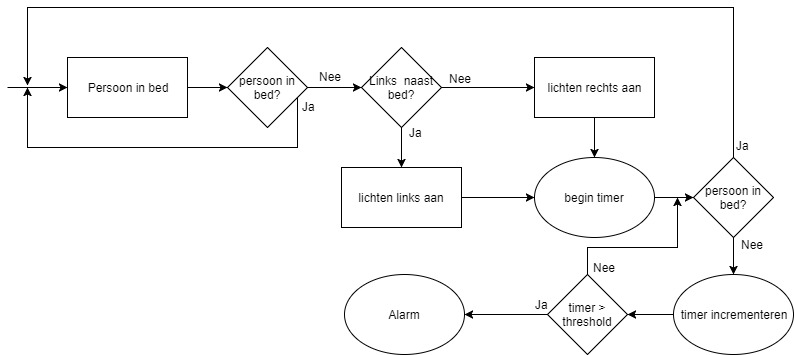
\includegraphics[scale=0.5]{HoogNiveauBlokDiagram}
	\caption{Werkingsschema op hoog niveau}
	\label{imgWeS}
\end{figure}
Dit onderzoek heeft als doel het ontwikkelen van een visiesysteem dat kan detecteren langs welke zijde een pati\"ent uit bed stappt en kan meten hoelang de pati\"ent wegblijft. Als mogelijke uitbereiding kunnen we ook val detectie toevoegen. In figuur \ref{imgWeS} is het werkingsschema op hoog niveau te zien.
We beginnen links bij persoon in bed. We gaan er vanuit dat er een persoon in het bed ligt.  Vervolgens gaan we testen of er delen van het lichaam zich uit het bed bevinden, op welke manier we dit doen, wordt later besproken in sectie ...... . Indien er een persoon in het bed gevonden wordt, blijven we deze test herhalen. Is er geen persoon in het bed gedetecteerd, gaan we kijken naar welke zijde. Vanaf het moment dat de persoon het bed heeft verlaten, wordt er een timer gestart. Vervolgens gaan we terug kijken of er een persoon in he bed is. Als er een persoon is, dan gaan we terug naar de startpositie. Als er geen persoon in het bed is, wordt de waarde van de timer ge\"incrementeerd. Daarna gaan we de waarde van de timer vergelijken met een threshold. Is de waarde van de teller groter dan de threshold, dan gaat er een alarm afgaan, deze persoon is te lang uit het bed. Indien de waarde van de timer kleiner is dan de threshold, gaan we terug nazien of er een persoon in het bed is.  De waarde van de threshold kan in het programma aangepast worden als het toilet zich ver van het bed bevindt.  Als de persoon terug in het beeld komt, stopt de teller en bevinden we ons weer in de eerste toestand.

\section{IR camera}
\label{MRefIRC}
Voor de uitwerking van ons project maken we gebruik van een infrarood camera. Deze hebben we eerder al besproken in onze literatuurstudie \ref{refIRC}. We gebruiken deze camera omdat deze ter beschikking werd gesteld door de school en dit ons ook een logische keuze leek. Dit omdat de persoon door de infraroodbeelden al minder snel herkenbaar zijn, op de beelden, wat een zeer belangrijk deel is van de specificaties. Verder is dit in verhouding met de andere besproken types van camera's in de literatuurstudie\ref{refTVC}, een goedkope camera. Verder is in onze toepassing het niet nodig om een gedetailleerd beeld van de pati\"ent te verkrijgen. Hierdoor is de constructie van IP en PTZ camera's hier niet van toepassing. Andere types van camera zouden ook kunnen gebruikt worden. Maar dit onderzoek, is door bovenvermelde redenenen, niet door ons gedaan. We bespreken de gebruikte camara, namelijk die Seek Thermal Compact in sectie \ref{mRefSTh}. Voor de plaatsing van onze camera hebben we een aantal berekeningen gedaan. Dit om te zien waar en op welke hoogte onze camera het beste geplaatst wordt. Deze berekeningen zijn te vinden in sectie \ref{mRefSTP}.

\subsection{Seek Thermal Compact}
\label{mRefSTh}

\begin{figure}[hbp]
	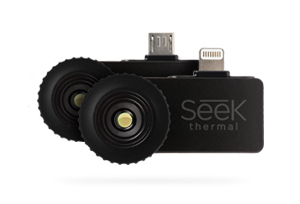
\includegraphics[scale=0.75]{SeekThermalCompac}
	\caption{Image of Seek Thermal Compact}
	\label{imgSTC}
\end{figure}
Dit is een zeer kleine camera die bedoeld is om te gebruiken met een Android smartphone of met een IPhone. Een afbeelding van de camera is terug te vinden in figuur \ref{imgSTC} \cite{bibImgSTC}. Wij hebben gebruik gemaakt van de versie die normaal op Android gestuurde systemen werkt. Om deze camera te kunnen gebruiken op een computer, hebben we gebruik gemaakt van code die ons beschikbaar is gesteld via Eavise \cite{bibSTC}. Via deze code kunnen we van de camera binnen halen en bekijken. Deze camera is gebruikt om alle testbeelden te maken tijdens de experimenten die besproken worden in hoofdstuk \ref{ERef}. Hieronder bespreken we de specificaties van de Seek Thermal Compact voor gebruik op Android toestellen \cite{bibImgSTC}: 
\begin{itemize}
	\item $\mu$USB Thermal Camera for Android devices
	\item Werkt met de meeste Android toestellen die werken met 4.3 of hoger. (Op de website, \url{http://www.thermal.com/products/compact/} is een lijst met compatibele modellen te vinden. 
	\item 206 * 156 Thermal Sensor
	\item 12 $\mu$ Pixel Pitch
	\item Vanadium Oxide Microbolometer
	\item Chalocogeninde Lens
	\item $36^{\circ}$ zicht
	\item Magnesium behuizing
	\item Lange golf infrarood 7.2 - 13 $\mu$m
	\item  spectrum van -40 tot 330 $^{\circ}$c
	\item 9Hz
	\item Bevat een waterdichte cover
	\item Model: UW-AAA
\end{itemize}
Een nadeel van deze camera is dat hij via een $\mu$USB connectie met de computer verbonden moet worden. Hierdoor mag de camera niet te ver staan van de computer waarop het programma met de gedragsanalyse draait, of er moet onderzoek gedaan worden naar een mogelijkheid om de beelden draadloos door te sturen.

\subsection {Plaatsing van de camera}
\label{mRefSTP}
Er zijn verschillende manieren, om de camera te plaatsen. Maar aangezien we het bed in de code moeten kunnen detecteren, willen we dat de positie van het bed hetzelfde blijft ten opzichte van de camera. Hierdoor moeten we een gebruik maken van een statische opstelling. Dit kunnen we doen door de camera via een constructie aan het bed te bevestigen. Een andere manier om een statische opstelling te verkrijgen, is door de camera te bevestigen aan het plafond of \'e\'en van de muren van de kamer.  We weten de openingshoek van de camera. Dankzij deze kunnen we de nodige hoogte van de camera berekenen. We nemen de lengte van het bed (2m) als de bepalende factor voor de hoogte. De camera mag altijd hoger bevestigd worden, zo gaat er meer van de omgeving waargenomen worden. 

\subsubsection{Camera recht boven hoofdeinde}
De eerste berekening die we doen, is een situatie waar de camera recht boven het hoofdeinde geplaatst is. Deze kan zowel via aan constructie aan het bed gemonteerd worden als rechtstreeks aan het plafond. De camera hangt in het midden van de breedte van het bed. Op afbeelding \ref{imgCBB} is een schets van de situatie te zien. 
\begin{figure}[hbp]
	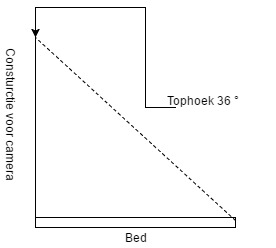
\includegraphics[scale=0.7]{CamBovenBed}
	\caption{Schets van camera recht boven bed}
	\label{imgCBB}
\end{figure}
De berekening van de hoogte is in dit geval heel eenvoudig. Het gaat hier over een rechthoekige driehoek. We kunnen her gebruikt maken van de goniometrische regels voor rechthoekige driehoeken.
\begin{displaymath}
tan(\alpha) =\frac{o}{x}
\end{displaymath}
\begin{displaymath}
tan(36^\circ) = \frac{2}{x}
\Rightarrow x = \frac{2}{tan(36 ^\circ)} = 2,75
\end{displaymath}
met
\begin{itemize}
	\item $\alpha$ is de openingshoek van de camera in uitgedrukt graden
	\item o is de lengte van het bed uitgedrukt in meter
	\item x is de gevraagde hoogte in meter
\end{itemize}
Uit de berekeningen blijkt dat de camera 2,75 meter boven het bed moet hangen. Dit is onmogelijk, omdat de gemiddelde kamer ongeveer een 2,5 meter hoog is. Hierdoor zullen we de camera moeten hangen op een andere locaties. Hieronder volgen de berekeningen voor de situatie waarbij de camera niet recht boven het hoofdeinde hangt.

\subsubsection{Camera niet recht boven hoofdeinde}
\begin{figure}[hbp]
	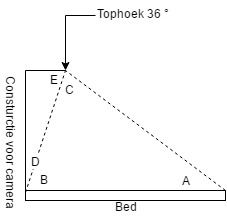
\includegraphics[scale=0.7]{CameraNietRechtBoven}
	\caption{Schets van camera niet recht boven bed}
	\label{imgCNRBB}
\end{figure}
Nadat we uit de voorgaande berekening hebben kunnen besluiten dat het onmogelijk is het bed volledig op het frame te krijgen als we de camera recht boven het hoofdeinde hangen. Gaan we de nodige hoogte bepalen als de camera boven het bed komt te hangen, maar niet recht boven het hoofdeinde. figuur \ref{imgCNRBB} geeft een schets weer van de situatie. De camera hang in het midden van de breedte van het bed. De drukletters in de figuur \ref{imgCNRBB} zijn de verschillende hoeken. Deze worden ook in de berekening gebruikt .Door te rekenen met hoeken in driehoeken en het gebruik van de sinusregels voor willekeurige- en rechthoekige driehoeken, kunnen we de gezochte hoogte berekenen. Alle hoeken worden uitgedrukt in graden en de lengtes in meter. Voor het horizontale gedeelte van de constructie nemen we een paar keer een andere waarde, zo kan u zien hoe de hoogte evolueert.
Bepaling waarden voor hoeken:
\begin{displaymath}
C=36^\circ
\end{displaymath}
\begin{displaymath}
B=E
\end{displaymath}
\begin{displaymath}
A + B + c = 180 ^\circ \rightarrow A = 144^\circ - E
\end{displaymath}
Vervolgens gaan we de sinusregel toepassen voor niet rechthoekige driehoeken:
\begin{displaymath}
\frac{2}{sin(36^\circ)} = \frac{s}{sin(144^\circ - E)}
\end{displaymath}
Door gebruik van de cosinusregel in de rechthoekige driehoek verkrijgen we:
\begin{displaymath}
cos(E) = \frac{x}{s}
\end{displaymath}
Uit de twee voorgaande formules kunnen we hoek E berekenen als we de waarde voor x kennen:
\begin{displaymath}
cos(E)sin(144^\circ-E) = \frac{x.sin(36^\circ)}{2}
\end{displaymath}
Nu we de waarde van de hoek E hebben bepaald, kunnen we door gebruik te maken van de tangens regel de hoogte berekenen:
\begin{displaymath}
h = tan(E)*x
\end{displaymath}
met:
\begin{description}
	\item [A, B, C, D, E] de hoeken zoals weergegeven in figuur \ref{imgCNRBB}
	\item[s] de schuine zijde in de driehoek (tussen B en C)
	\item[x] de horizontale afstand tussen het hoofdeinde en de plaats van de camera
	\item[h] de hoogte waarop de camera moet komen
\end{description}
Een overzicht van de berekende waarden, is terug te vinden in tabel \ref{refTabCNRBB}. Uit deze waarden kunnen we besluiten dat het onmogelijk is om deze camera in een normale ruimte aan het bed te bevestigen.
\begin{table}[hbp]
	\caption{Berekende waarden voor camera niet recht boven hoofdeinde}
	\begin{tabular}{|c|c|c|}
		\hline
		x & E & h \\ \hline
		0.1 & 88 & 2.86 \\ \hline
		0.25 & 85 & 2.85 \\ \hline
		0.5 & 81 & 3.15 \\ \hline
		0.75 & 76 & 3.01 \\ \hline
		1 &  72 & 3.08 \\
		\hline
	\end{tabular}
	\label{refTabCNRBB}
\end{table}

\subsubsection{Camera niet bevestigd aan het bed}
De voorgaande berekeningen hebben ons getoond dat we de camera niet aan het bed kunnen monteren. Nu gaan we de hoogte berekenen die we nodig hebben, als de camera achter het bed tegen de muur hangt, op een afstand van het voeteneinde. Een schets van de situatie is terug te vinden in de afbeelding \ref{imgCNB}. 
\begin{figure}[hbp]
	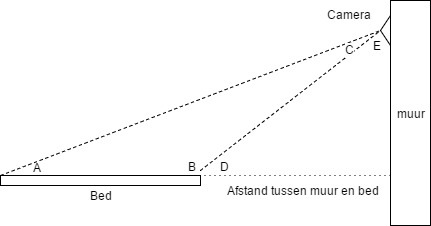
\includegraphics[scale=0.7]{CameraNietAanBed}
	\caption{Schets van camera niet bevestigd aan bed}
	\label{imgCNB}
\end{figure}
Net zoals bij de vorige berekening vindt u de namen van de hoeken terug in de afbeelding. Bij deze berekening nemen we aan dat de camera zelf geen dikte heeft. Dus de hoek E zit tussen de denkbeeldige lijn die de openingshoek van de camera weer geeft en de muur. Dit om de berekeningen iets eenvoudiger te houden. 
Over de hoeken hebben we volgende gegevens:
\begin{displaymath}
C=36^\circ
\end{displaymath}
\begin{displaymath}
A+B+C = 180^\circ
\end{displaymath}
\begin{displaymath}
B + D = 180^\circ \Rightarrow A = D-36^\circ
\end{displaymath}
Uit de sinus regel voor niet rechthoekige driehoeken kunnen we volgende formule afleiden:
\begin{displaymath}
\frac{2}{sin(36^\circ)}=\frac{s}{sin(D-36^\circ)}
\end{displaymath}
Door de cosinusregel in rechthoekige driehoeken, geldt volgende formule
\begin{displaymath}
cos(D)=\frac{x}{s}
\end{displaymath}
Uit de twee voorgaande formules kunnen we de waarde van D berekenen als we de waarde voor x kennen:
\begin{displaymath}
cos(D)sin(D-36 ^\circ)=\frac{x . sin(36^\circ)}{2}
\end{displaymath}
Vervolgens gaan we de tangens regel voor rechthoekige driehoeken gebruiken om h te bepalen:
\begin{displaymath}
h=tan(D) . x
\end{displaymath}
met:
\begin{description}
	\item [A, B, C, D, E] de hoeken zoals weergegeven in figuur \ref{imgCNRBB}
	\item[s] de schuine zijde in de driehoek (tussen B en C)
	\item[x] de afstand tussen het bed en de muur
	\item[h] de hoogte waarop de camera moet komen
\end{description}
Een overzicht van de berekende waarden, worden weergegeven in tabel \ref{refTabCNB}.

\begin{table}[hbp]
	\caption{Berekende waarden camera niet aan bed bevestigd}
	\begin{tabular}{|c|c|c|}
		\hline
		horizontaal & D & hoogte \\ \hline
		0.25 & 84 & 2.37 \\ \hline
		0.5 & 77 & 2.16 \\ 
		\hline
	\end{tabular}
	\label{refTabCNB}
\end{table}
Aangezien een kamer ongeveer 2,5 meter hoog is, zien we dat het mogelijk is de camera op een hoogte te plaatsten waardoor het volledige bed zichtbaar is.

\subsubsection{Besluiten bij de berekeningen}
Uit de eerste twee berekeningen besluiten we dat het onmogelijk is om de gebruikte camera aan het bed te bevestigen en heel het bed te zien. Er zijn twee mogelijke oplossingen. We kunnen een andere camera nemen met een grotere openingshoek, of we kunnen de camera verder van het bed plaatsen zodat de benodigde hoogte kleiner gaat worden.\\
Uit de tweede berekening kunnen we besluiten dat het met de gebruikte camera wel mogelijk is om het volledige bed in het frame te krijgen. Als we de camera achter het bed aan de muur hangen.

\section{Gebruikte technieken voor de gedragsanalyse}
\label{MRefMGA}
Deze sectie is opgebouwd uit twee verschillende delen. In het eerste deel bespreken we de dingen de we als eerste hebben gedaan in dit onderzoek, nog voor we begonnen zijn aan de effectieve gedragsanalyse. In het tweede deel bespreken we de gebruikte technieken aan de hand van de verschillende fasen in het werkingsschema, dat terug te vinden is in figuur \ref{imgWeS} en dat we hebben besproken in sectie \ref{MRefWeS}. Voor het maken van de gedragsanalyse en de code die we schrijven tijdens de voorbereidende technieken, wordt gebruik gemaakt van openCV, de gebruikte taal voor de code is c++.

\subsection{Voorbereidende technieken}
Voor we begonnen zijn aan de gedragsanalyse, hebben we eerst bekeken of we de camera met de gekregen code, aan de praat kregen op de computer. Vervolgens hebben we nagekeken of we met deze camera een persoon in een bed kunnen waarnemen. Nadien hebben we twee klassen geschreven. De eerst is SaveImage, deze heeft \'e\'en methode (saveImage) en heeft als doel het frame dat we ophalen met de gekregen code, weg te schrijven op het door ons gedefini\"eerde pad. De tweede geschreven klasse is de klasse GetImages. Deze heeft eveneens \'e\'en methode, namelijk getImage. Deze methode dat het frame op het door ons opgegeven pad weer ophalen. Deze technieken zijn gebruikt in het eerste experiment, meer informatie hierover is te vinden in sectie \ref{ERefOvB}. Tijdens deze fase van het onderzoek hebben we eveneens de camera op de juiste hoogte in de kamer gemonteerd zodat het bed volledig in het frame past. 

\paragraph{Opmerkingen}
openCV beschikt over standaardfunctie voor het wegschrijven en ophalen van afbeeldingen. Wij gebruiken deze, maar hebben de twee klassen geschreven omdat er voor het opslaan van de afbeelding een conversie moet gebeuren om de afbeeldingen om te zetten naar het juiste bestandstype. Anders zouden we de conversie elke keer apart moeten oproepen. Het bespaart elke keer een paar lijnen code en we verkleinen eveneens de kans dat iemand het vergeet of er een fout in getypt worden.\\
Nadat deze fase afgelopen was, hebben we de Klassen SaveImages en GetImages samengevoegd tot \'e\'en klasse, namelijk SGImage. De twee methodes worden vervolgens voor deze klasse ge\"implementeerd. Dit omdat we nu nog maar \'e\'en object moeten aanmaken om zowel afbeeldingen op te slaan als terug op te halen. Dit is effici\"enter. \\
Het opslaan en ophalen van de afbeeldingen is ook nodig voor het maken van opeenvolgende tesbeelden. Zo kunnen we overdag de ontwikkelde technieken laten lopen over dezelfde beelden en hier besluiten uit trekken. Verder maakt dit dat we ook niet elke keer als we iets willen testen we een persoon moeten zoeken die dan even in een bed wilt gaan liggen.

\subsection{Ontwikkelen van de gedragsanalyse}
Zoals eerder aangehaald, gaan we de gebruikte methodes van dit deel van het onderzoek overlopen aan de hand van het werkingsschema. Dit is terug te vinden in afbeelding \ref{imgWeS}. De gebruikte technieken zijn terug te vinden in de volgende paragrafen.

\subsubsection{Persoon in bed}
\begin{figure}[hbp]
	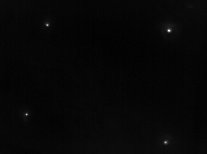
\includegraphics[scale=0.75]{SeekCamBed}
	\caption{Foto van het bed met warme objecten op de hoeken}
	\label{imgCBe}
\end{figure}
Het eerste blokje in het werksschema is persoon in bed. We hebben een klasse Bed gemaakt. Een object van de klasse bed bestaat uit acht integers. Dit zijn de co\"ordinaten van de hoekpunten van het bed. Dankzij deze kunnen we achteraf bepalen of een persoon in bed ligt, of aanstalten maakt om eruit te komen. Verder hebben we in dit stadium ook een mousecallback functie gemaakt deze wordt besproken in de eerstvolgende paragraaf, daarna volgt een bespreking van de Bed klasse \\

\paragraph{mouseCallBack functie}
 De functie gaat de punten waarop geklikt wordt met de linkermuisknop opslagen in een vector. Door een klik met de rechtermuisknop, wordt het laatste punt in de vector verwijdert. Door op enter te klikken wordt de functie be\"eindigd. 
 
\paragraph{klasse Bed}
De klasse bezit drie costructoren. De eerste heeft geen argumenten. Indien deze opgeroepen wordt is het bed object een punt. De tweede constructor, heeft acht integers als argument. De derde methode heeft twee argumenten. Het eerste is een afbeelding en het tweede is een integer. De afbeelding is een frame waarop een leeg bed te zien is, waar op elke hoek van het bed een warm object geplaatst is. Een voorbeeld van zo een afbeelding is te zien in figuur \ref{imgCBe}. De camera gaat de warme objecten weergeven als lichte punten op een donkere achtergrond. Het tweede argument, de integer gaat bepalen op welke manier de co\"ordinaten van de lichtere punten in de afbeelding toegekend worden aan de integers van het bed object. Als de integer 0 is, dan wort er via de mouseCallBack functie,die eerder is besproken, gevraagd om de hoekpunten van het bed aan te klikken, beginnend bij het hoekpunt rechtsboven. Op elk punt moet dan \'e\'en keer gelkikt worden. De klik positie wordt toekend aan het bed object. Als de integer van het argument een andere waarde heeft als 0. Dan worden de locaties van de punten via blobdetectie automatisch uit de afbeelding opgehaald en toegekend.\\
\begin{figure}[hbp]
	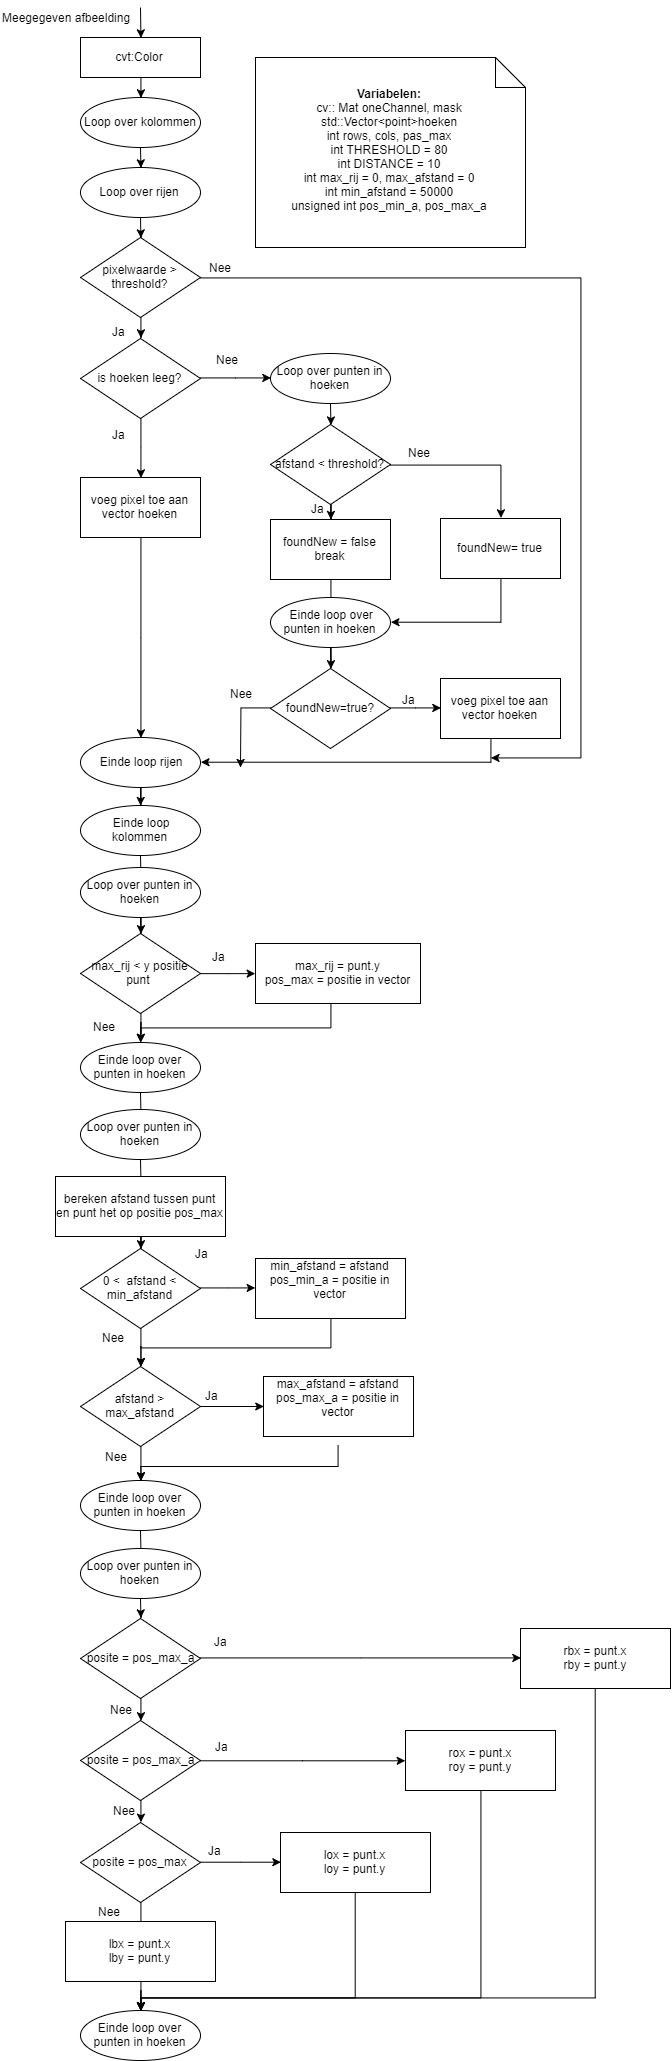
\includegraphics[scale=0.34]{FlowChart_setValuesAuto}
	\caption{Flowchart van de methode setValuesAuto}
	\label{imgFCSVA}
\end{figure}
De klasse bed heeft een aantal andere methodes, de eerste is setValues deze heeft acht integers als argument en gaat deze toekennen aan de integers van het object. Een andere methode is seValuesImg, deze gaat via de mouseCallBack functie de waarden van de co\"ordinaten toekennen aan het object. setValuesAuto gaat automatisch de hoepkunten bepalen aan de hand van de weergegeven afbeelding. de flowchart van deze methode is te zien in figuur \ref{imgFCSVA}. De methode werkt als volgt, er wordt een lege vectorgecre\"erd. Vervolgens lopen we over alle pixels in de afbeelding, als de pixel licht is, wordt er gezien of we de waarde aan de vector moeten toevoegen. De pixelwaarde moet toegevoegd worden als de vector nog leeg is, of als er geen punt in de directe omgevint in de vector staat. Als we door alle pixels hebben gelopen, gaan we bepalen welk punt het meest onderaan staat. Dit is de linker onderhoek. Door gebruikt te maken van de onderlinge afstand van dit punt met de drie andere punte in de vector, worden de waarden aan de juiste hoeken tegekend. Een ander methode is sidesOfBed. Deze methode gaat aan de hand van de hoeken van het object, de zijkanten van het bed bepalen. Dit zijn twee vergeljkingen van rechten. De co\"effici\"enten van deze vergelijkingen worden in een vector terug gegeven. 




\subsection{Detect}
\label{mRefDet}
In deze klasse worden de detectie van het uit het bed stappen gedaan. Om een object van de klasse Detect te maken, moet je een object van de klasse Bed toewijzen. De klasse Detect bevat twee constructoren. Deze worden eerst besproken. Vervolgens bespreken we de verschillende methodes van deze klasse. De eerste methode is createMask, de tweede is checkMovement, de volgende is checkBed, hierna is er ook nog de tempDifference methode, als voorlaatste is er de createMaskNew methode en om af te sluiten hebben we de erDil methode.

\subsubsection{Constructoren}
De klasse heeft 2 verschillende contructoren, namelijk een afbeelding als argument of acht integers als argument.

\paragraph{Afbeelding als argument}
De eerste constructor van de klasse heeft een afbeelding als argument. We  roepen de methode setValuesAuto van de klasse bed op. Zo krijgt het bed object van de klasse de juiste co\"ordinaten voor de hoekpunten. 

\paragraph{Acht integers als argument}
De tweede constructor heeft acht integers als argument. Met deze waarden wordt de methode setValues van het bed object opgeroepen.

\subsubsection{createMask}
\begin{figure}[hbp]
	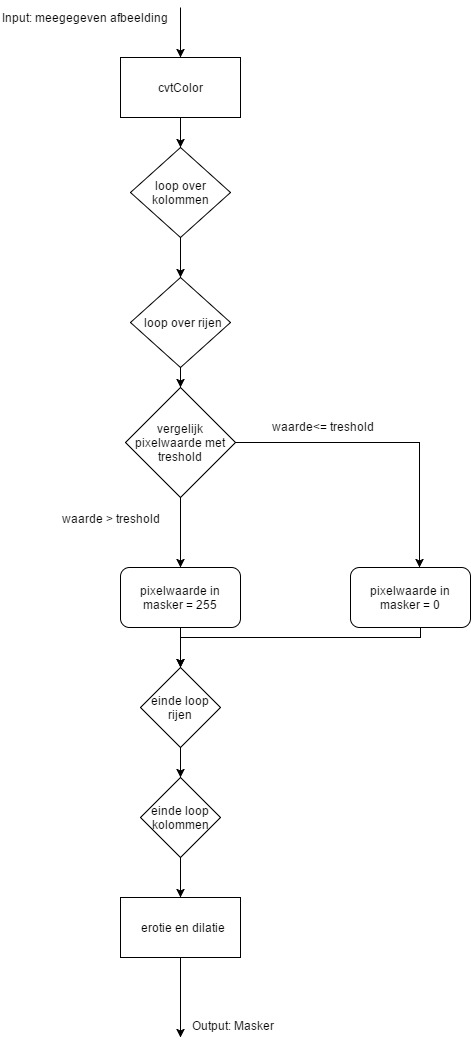
\includegraphics[scale=0.45]{FlowShart_createMask}
	\caption{Flowchart van de methode createMask}
	\label{imgFSCMa}
\end{figure}

Deze methode heeft als doel het maken van het masker. We leggen het werkingsprincipe van de methode uit aan de hand van een flowchart. Deze ziet u in figuur \ref{imgFSCMa}. Het principe is heel eenvoudig, als argument wordt er een afbeelding meegegeven. De afbeelding die we inlezen is 3 kanaal. Daarom zetten we de afbeelding eerst om naar een 1 kanaal afbeelding. Dit is de eerste rechthoek in onze flowchart.  Deze wordt vervolgens  pixel per pixel doorlopen. Als de waarde op de bewuste pixel groter is dan de threshold wordt de overeenkomende pixel in het masker wit gemaakt, De rest blijft zwart. Dit wordt ook gedaan zodat de persoon in de beelden onherkenbaar zou zijn. Het masker wordt terug gegeven. De door ons gebruikte drempelwaarde heeft een waarde van 180 gekregen. Nadat de rijen en kolommen zijn doorlopen wordt er erosie en dillatie toegepast, dit is het laatste rechthoekje in de figuur. Vervolgens wordt het masker terug gegeven.  Een voorbeeld van een meegegeven afbeelding en een teruggekregen masker ziet u in figuur \ref{imgCMa}.

\begin{figure}[hbp]
	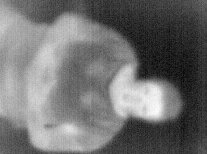
\includegraphics[scale=0.75]{EersteExperiment_img0}
	
\includegraphics[scale = 0.75]{EersteExperiment_mask0}
	\caption{Voorbeeld van masker: (links) meegegeven afbeelding (rechts) verkregen masker}
	\label{imgCMa}
\end{figure}

\subsubsection{checkMovement}
Deze methode gaat 2 opeenvolgende frames vergelijken om te zien of het de moeite is om de volgende zwaardere berekeningen te doen. Indien er geen beweging is geweest, kan de persoon ook niet uit bed gestapt zijn, of eruit gevallen. Deze methode heeft als argument 2 opeenvolgende frames. Deze worden pixel per pixel vergeleken. Het aantal pixels waar er een verschillende waarde is wordt bijgehouden. Deze wordt vergeleken met een drempelwaarde. Indien het aantal verschillende pixels kleiner is dan de drempelwaarde, is er geen beweging geweest en wordt false terug gegeven. Indien er wel meer verschillende pixelwaarden zijn, heeft de persoon bewogen en wordt er true terug gegeven.

\subsubsection{checkBed}
\begin{figure}[hbp]
	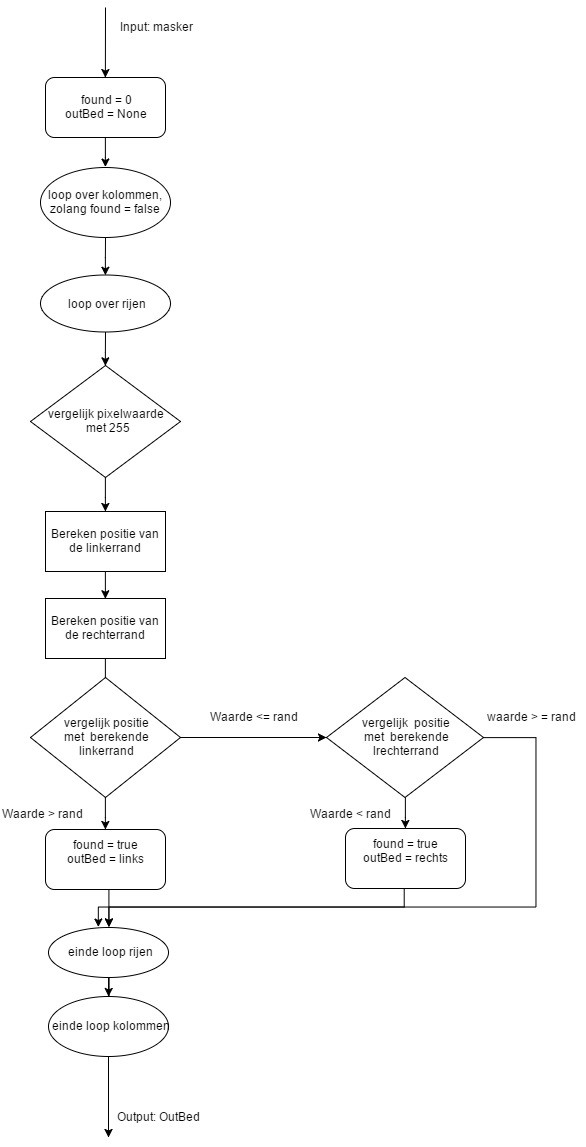
\includegraphics[scale=0.45]{FlowShart_checkBed}
	\caption{Flowchart van de methode checkBed}
	\label{imgFCCBe}
\end{figure}
Deze methode wordt verduidelijkt aan de hand van een flowchart. Deze vindt u terug in figuur \ref{imgFCCBe}. De methode checkBed heeft \'e\'en argument, namelijk een afbeelding. Als je deze methode oproept, geef je het masker mee dat door de methode createMask gemaakt werd. In deze methode gaat men kijken of er delen die door het masker aangeduid werden als pati\"ent uit het bed steken. \\
We gaan voor elke kolom kijken. Als er een witte pixel gevonden is, gaat men eerst bekijken waar deze licht ten opzichte van de linkse bedrand. Die kan je halen uit de vergelijkingen die bepaald worden door sidesOfBed in de klasse bed. Als de waarde groter is, dan is er daar een lichaamsdeel over de bed rand. Er wordt terug gegeven dat er links uit het bed gestapt wordt. Indien de waarde kleiner is gaat men vergelijken met de y-waarde van de rechter bed rand. Heeft de gevonden y waarde een grotere waarde dan die van de rechter bed rand, dan stapt de persoon langs rechts uit bed. Indien de y-waarde tussen de bedranden blijft, gebeurt er niets.

\subsubsection{tempDifference}
\begin{figure}[hbp]
	\includegraphics[scale=0.45]{FlowChart_TempDifference}
	\caption{Flowchart van de methode tempDifference}
	\label{imgFCTDi}
\end{figure}
Deze methode is toegevoegd na het uitvoeren van het tweede experiment \ref{ERefDUB} en het maken van onze conclusies hieruit \ref{ERefDBB}. Deze methode heeft veel weg van de checkMovement methode die we hierboven hebben besproken. Om de werking van de methode te verduidelijken, hebben we een flowchart toegevoegd in figuur \ref{imgFCTDi}. In deze methode berekenen we temporeel verschil zoals besproken bij voorgrond /achtergrond segmentatie \ref{refBET}. Er wordt een afbeelding teruggegeven waarbij alle pixels nul als waarde hebben, buiten de pixels waar de waarde niet hetzelfde is voor de twee opeenvolgende frames, die pixel heeft de waarde 255.Een voorbeeld van het resultaat, dat ik vanaf nu bewegingsMasker noem, vindt u in figuur \ref{imgBMa}. \\
Deze extra stap wordt gedaan om te vermijden dat warmere vlekken van de achtergrond verward worden met lichaamsdelen van een persoon.
\begin{figure}[hbp]
	
\includegraphics[scale=0.75]{bewegingsMatrix}
	\caption{Voorbeeld van een bewegingsmasker}
	\label{imgBMa}
\end{figure}

\subsubsection{createMaskNew}
\begin{figure}[hbp]
	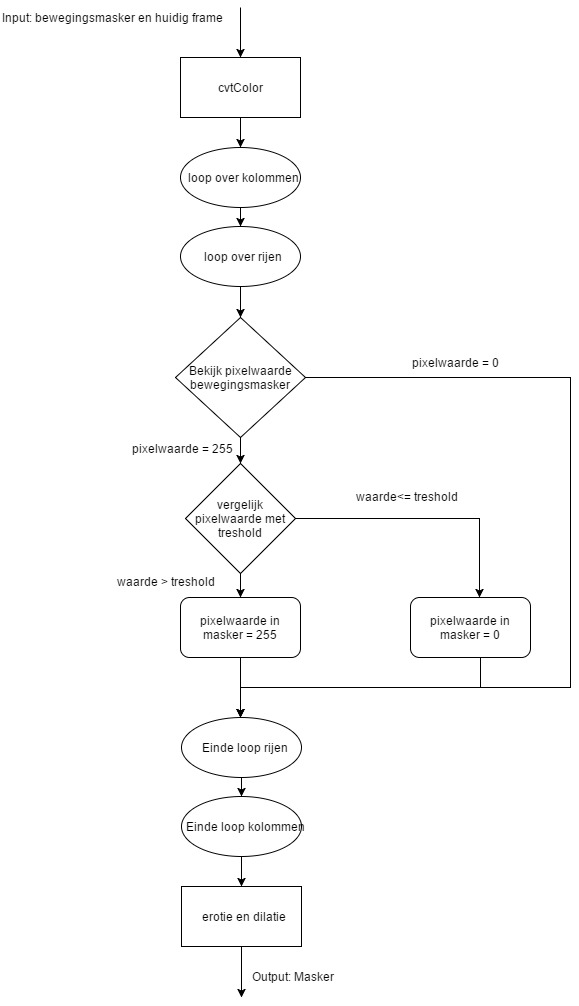
\includegraphics[scale=0.45]{FlowChart_createMaskNew}
	\caption{Flowchart van de methode createMaskNew}
	\label{imgFCCMN}
\end{figure}
Om het werkingsprincipe van deze methode te verduidelijken, hebben we een flowchart toegevoegd. Deze vindt u in figuur \ref{imgFCCMN}. Zoals u uit deze figuur en uit figuur \ref{imgFSCMa} kunt afleiden, lijkt deze methode op de reeds besproken methode createMask. Dit komt doordat dit een nieuwere, verbeterde versie is van createMask. Deze methode heeft twee argumenten, namelijk het huidige frame en het bewegingsmasker, dat als resultaat uit de methode tempDifference komt. We gaan opnieuw \'e\'en voor \'e\'en over alle pixels lopen en bekijken het bewegingsmasker, is de waarde voor de huidige pixel gelijk aan 255, dan bekijken we het meegegeven frame. Is de pixel waarde van het frame groter dan de threshold, dan wordt de pixelwaarde van het terug gegeven masker 255. Anders blijft de pixelwaarde nul. Voor we het berekende masker gaan terug geven gaan we nog eroderen en vervolgens dilleren, dit om de mogelijk kleine afwijkingen te elimineren, zodat er geen valse detecties gebeuren. Hiervoor gebruiken we de methode erDil die besproken wordt in de volgende paragraaf. Een voorbeeld van een masker dat terug gegeven wordt en het originele frame vindt u terug in figuur \ref{imgCMN}.
\begin{figure}[hbp]
	
\includegraphics[scale=0.65]{MaskMetDif}
	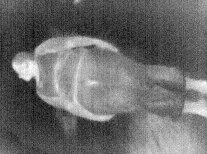
\includegraphics[scale=0.65]{ImgMetDif}
	\caption{Frame en masker gemaakt met methode createMaskNew}
	\label{imgCMN}
\end{figure} 
 
 \subsubsection{erDil}
Deze methode heeft twee argumenten. De eerste is de afbeelding waarop de erosie en dillatie toegepast moet worden. Het tweede is de grootte van de matrix gebruikt voor het eroderen en dilleren. Hoe groter de waarde, hoe meer details er van de afbeelding verdwijnen. Nadat de erosie en dillatie, wat men ook wel openen noemt, is toegepast wordt de resultaatafbeelding terug gegeven. 
 
 \subsubsection{tempDifferenceNew}
Deze methode is een verbetering van het bewegingsmasker. Deze methode heeft als doel een oplossing te bieden voor het probleem van de restwarmte. We gaan ook hier weer twee opeenvolgende frames met elkaar vergelijken. Als de pixelwaarde van het huidige frame min de pixelwaarde van het vorige frame groter is, dan wordt de pixelwaarde van het bewegingsmasker 255. Waarom enkel als de waarde groter is? Omdat de persoon normaal het warmste deel van het beeld moet zijn. Hierdoor zal dus de beweging van de persoon gepaard gaan met het stijgen van de pixelwaarde. De dalende pixelwaarden zijn bijvoorbeeld het afkoelen van het bed nadat de persoon eruit is gestapt en hebben we verder niet meer nodig.
 
 \subsection{DetectNotNotmalized}
 \label{mRefDNN}
Deze klasse is afgeleid van de eerder besproken Detect \ref{mRefDet} klasse. Deze klasse is gemaakt om te werken met live beelden en zonder normalisatie. Deze klasse heeft \'e\'en methode. Namelijk createMask.
 
 \subsubsection{createMask}
 Deze methode is ongeveer het zelfde als de eerder verklaarde gelijknamige methode. Het grootste verschil is dat doordat je met live beelden werkt je de cvtColor stap niet nodig hebt. Het doel is nog altijd het zelfde, namelijk het cre\"eren van een masker dat wit is op de plaatsten waar er een persoon gedetecteerd wordt en de overige pixels zwart zijn. Voor deze methode is er geen nieuwe flowchart toegevoegd. U kan kijken naar die van createMask van de klasse Detect, figuur \ref{imgFSCMa}. U dient dus enkel de cvtColor stap over te slaan. 
 
\subsection{Gebruikte functies}
\label{MRefGFu}
Buiten de gebruikte klassen en hun methoden, is er eveneens een functie die tot de namespace LibSeek behoort.

\subsubsection{MouseCallBack}
Deze functie wordt bijvoorbeeld opgeroepen in de constructor van Bed als je deze oproept met een afbeelding als argument. De functie gaat de punten waarop geklikt wordt met de linkermuisknop opslagen in een vector. Door een klik met de rechtermuisknop, wordt het laatste punt in de vector verwijdert. Door op enter te klikken wordt de functie be\"eindigd. 

\subsection{Test Programma's}
\label{mRefTPr}
Er zijn verschillende testprogramma's geschreven. Dit telkens om aparte klassen en hun methodes te testen en eventuele optimalisaties toe te passen. We werken met zoveel verschillende test programma's omdat we het project stap voor stap hebben opgebouwd. We zijn zeer eenvoudig begonnen met het opslagen en ophalen van afbeeldingen. Vervolgens hebben we eerst een masker gemaakt, daarna zijn we begonnen met het detecteren van bewegingen, het aanmaken van bedobjecten. Daarna zijn we verschillende methoden voor detectie van uit bed stappen afgegaan en hebben deze getest. Per afgewerkte fase is er telkens een ander testprogramma.

\subsection{Uiteindelijke programma's}
\subsubsection{saveBed}
saveBed is het programma dat we hebben gemaakt om het frame van het bed op te slaan. In dit programma gaan we maar \'e\'en frame van de Libseek Thermal camera ophalen. Dit frame wordt opgeslagen in de speciaal aangemaakte map voor de bedden. Je moet dit programma niet dagelijks laten lopen. Je moet dit enkel doen als de camera of het bed verplaatst is geweest, of er reden is om te geloven dat de opgeslagen hoekpunten van het bed niet correct zijn. Natuurlijk moeten de warme objecten op voorhand op de hoekpunten geplaatst worden. Dit programma maakt gebruik van de klasse SaveImage en haar methode.

\subsection{Programma} 
Programma is de laatst werkende versie van het programma en al zijn functionaliteiten. Er wordt gebruik gemaakt van alle bovenstaande klassen. De gebruikten methoden varieerden gedurende de verschillende experimenten. Een bespreking van de verschillende gebruikte methoden vindt u terug in het volgende hoofdstuk \ref{ERef}.

\chapter{Experiment}
\label{ERef}
Er hebben doorheen het jaar, verschillende experimenten plaats gevonden. We zijn begonnen met meer eenvoudige experimenten en zijn geeindigd met de moeilijkere experimenten. We bespreken de experimenten in chronologische volgorde. Na de beschrijving en de uitwerking van de verschillende experimenten worden conclusies getrokken uit de resltaten en de berekeningen. Met de conclusies van de vorige experimenten werd dan ook rekening gehouden bij de uitvoering van de volgende experimenten. Er zijn vier verschillende experimenten gebeurd. We beginnen met opslaan van beelden \ref{ERefOvB}. Vervolgens detecteren we het uit het bed stappen \ref{ERefDUB}. Dit deel is opgeslitst in twee verschillende experimenten, nameelijk een eerst poging \ref{ERefDUBEP} en een tweede poging \ref{ERefDUBTP}. Als laatste experiment werken we met live beelden \ref{ERefELB}.

\section{Opslaan van beelden}
\label{ERefOvB}
Dit eerste experiment bespreken we in 4 verschillende delen. We beginnen met te verklaren wat ons doel was van het experiment \ref{ERefOBD}, daarna bespreken we de gebruikte klassen, methodes en het flowchart \ref{ERefOBF}. Vervolgens verklaren we de speciefieke uitwerking van het experiment \ref{ERefOBU}. Als laatste trekken we onze conclusies \ref{ERefOBB}.

\subsection{Doel van het experiment}
Het doel van dit experiment is het opslagen van beelden. Dit om dan achteraf verschillende processen over de beelden te laten lopen en zo te zien welke de beste resultaten geeft.
\label{ERefOBD}

\subsection{Gebruikte klassen en flowchart}
\label{ERefOBF}
Voor dit expermiment werd voornamelijk de gekregen code geruikt om de code met de computer in te lezen. Vervolgens maken we gebruik van de klassen SaveImages \ref{mRefSIm}, GetImages \ref{mRefGIm} en Detect \ref{mRefDet}. De opeenvolging van de gebruikte methodes vindt u terug in het flowchart. 

\subsection{Uitvoering experiment}
\label{ERefOBU}
\begin{figure}[h]
	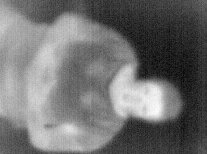
\includegraphics[scale=0.65]{EersteExperiment_img0}
	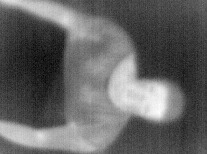
\includegraphics[scale=0.65]{EersteExperiment_img2}
	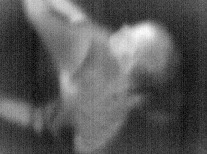
\includegraphics[scale=0.65]{EersteExperiment_img3}
	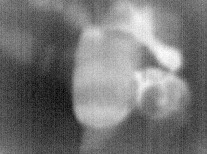
\includegraphics[scale=0.65]{EersteExperiment_img6}
	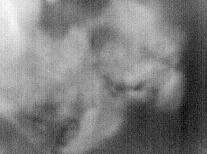
\includegraphics[scale=0.65]{EersteExperiment_img9}
	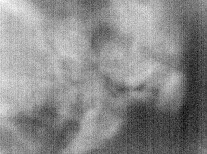
\includegraphics[scale=0.65]{EersteExperiment_img10}
	\caption{Opgeslagen beelden in eerste experiment}
	\label{imgEEx}
\end{figure}
Tijdens het eerste experiment hebben we overdag met behulp van de camera \ref{mRefSTh} beelden genomen van een persoon in bed. Hiervoor gebruiken we voornamelijk de klasse SaveImages \ref{mRefSIm}. Al gaan we hier maar om de 50 frames opslaan. Deze beelden kunnen we dan gebruiken voor het maken van bijvoorbeeld het masker en het verder afwerken van de detectie. Verder hebben we tijdens het maken van de beelden er ook op gelet dat de persoon verschillende slaaphoudingen aannam. Zo kunnen we nagaan of er een goede segementatie gebeurde vooralleer we begonnen met het maken van beelden gedurende een volledige nacht.\\
De beelden die zijn opgeslagen tijdens dit eerste experiment vindt u terug in figuur \ref{imgEEx}. Zoals u ziet hebben we zoveel mogelijk verschillende slaaphoudingen aangenomen. We zien eveneens een verschil in de afbeeldingen bij gebruik van een deken. De twee laatste afbeeldingen zijn van het leeg bed net nadat de foto's gertokken zijn. \\
Tijdens dit experiment hing de camera boven het bed. Een schets van het zijaanzicht van de situatie vindt u in afbeelding \ref{imgEEx2}. De oranje rechtoeken zijn de muren, plafond en grond van de kamer. Het paarse driehoekje is de camera. De camera hing boven het hoofdeinde van het bed, ongeveer in het midden van de breedte van het bed. \\
\begin{figure}[h]
	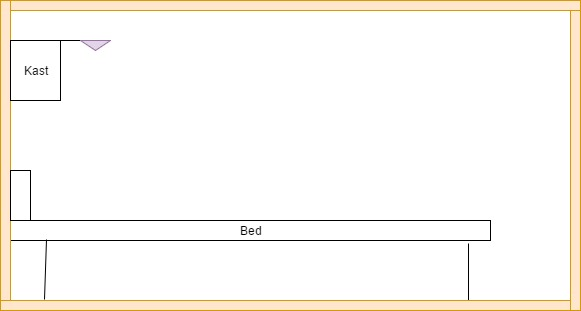
\includegraphics[scale=0.5]{SchetsExperiment1}
	\caption{Schets van de situatie in het eerste experiment}
	\label{imgEEx2}
\end{figure}
De foto's werden opgeslagen in de gewenste map.Verder zien we dat de persoon duidelijk te scheiden is van de achtergrond. Alleen zouden we de camera verder van het bed moeten plaatsen om meer van het bed op de beelden te kunnen zien. Door gebruik te maken van deze afbeeldingen, zochten we ook naar de ideale waarde voor de drempelwaarde om het masker te cre\"eren, zoals reeds besproken is bij de verschillende methodes van de klasse Detect \ref{mRefDet}.

\subsection{Besluiten uit het experiment}
\label{ERefOBB}
 Bij het bekijken van de opgeslagen beelden \ref{imgEEx} viel er ons iets op. Als er een deken over de persoon ligt, was hiervan enkel nog het hoofd en eventueel ook armen zichtbaar. Verder warmt het bed zeer snel op. Zo kan je in de laatste frames een leeg bed zien nadat de persoon er voor ongeveer 10 minuten had ingelegen. Dit is ook al zeer licht en kan leiden tot valse persoon detecties, dit is natuurlijk niet wenselijk voor ons experiment. Hiervoor gaan we dus in de komende experimenten een oplossing moeten zoeken. Het resultaat van het verkregen masker, vindt u in figuur \ref{imgCOB}.
\begin{figure}[h]
	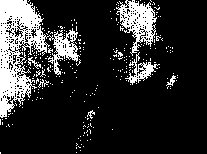
\includegraphics[scale = 0.75]{EersteExperiment_mask10}
	\caption{Verkregen masker voor leeg opgewarmd bed}
	\label{imgCOB}
\end{figure}
Ook ziet u dat als de persoon eerst op de zij heeft gelegen en gedraaid is een lichter vlak op de plaats waar de persoon voordien lag.
Een tweede mogelijk probleem dat optreedt is dat als je het masker cre\"eert, je de lichaamsdelen die bedekt worden door een deken maar ook door bijvoorbeeld een kledingstuk zoals pyama soms mist. Hierdoor zou het kunnen dat mogelijke aanstalten om uit het bed te stappen niet gedetecteerd worden. \\
Verder maakt de camera ook een klikgeluidje elke keer als er een frame gemaakt wordt. Dit kunnen sommige mensen hinderlijk vinden als ze hier mee moeten slapen. Dit kan enkel opgelost worden door een andere camera te gebruiken.  

\section{Detecteer uit bed stappen}
\label{ERefDUB}
Net zoals bij het voorgaande experiment \ref{ERefOvB} bespreken we ook dit tweede experiment in drie verschillende delen. We beginnen met het doel van het experiment \ref{ERefDBD} en het verduidelijken van de gebruikte klassen en methodes \ref{ERefDBK}. Vervolgens verklaren we de uitwerking \ref{ERefDBV} en als laatste nemen we een paar besluiten uit de verkregen beelden \ref{ERefDBB}. 

\subsection{Doel van het experiment}
\label{ERefDBD}
Het doel van het experiment is te bepalen of het mogelijk is te detecteren wanneer een person uit bed stapt. En het ontwikkelen van de algoritmes die hiervoor nodig zijn. 

\subsection{Gebruikte klassen en flowchart}
\label{ERefDBK}
Er wordt hier verder gebouwd op het voorgaande experiment \ref{ERefOvB}. Daarom maken we gebruik van dezelfde drie klassen, namelijk: SaveImages \ref{mRefSIm}, GetImages \ref{mRefGIm} en Detect \ref{mRefDet}. Hiernaast wordt tijdens dit experiment ook gebruik gemaakt van de klasse Bed \ref{mRefBed}. Het flowcharts van de experimenten zoals weergegeven in figuur \ref{imgFCDUBEP} en figuur \ref{imgFCDUBTP} tonen de opeenvolging van de gebruikte methodes.

\subsection{Verklaring uitwerking van het experiment}
\label{ERefDBV}
\begin{figure}[h]
	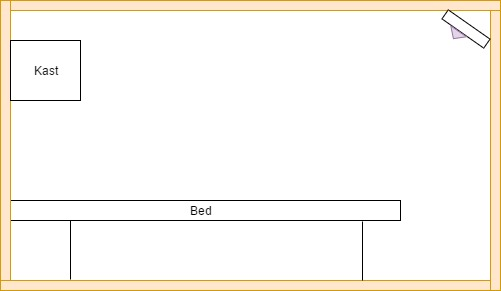
\includegraphics[scale=0.6]{SchetsExperimentTwee}
	\caption{Schets van het tweede experiment}
	\label{imgTEx}
\end{figure}
Eens de persoon uit de beelden gehaald kon worden. Hebben we nieuwe beelden gemaakt. Dit waarbij de hoeken van het bed gedefinieerd werden door middeel van de conrstuctor met een afbeelding \ref{mRefBed}. Daarna maakte de persoon verschillende keren aantstalten om uit het bed te stappen en hebben we nagegaan dat ons programma de juiste kant kan detecteren. \\
Voor dit experiment werd een nieuwe opstelling gemaakt. Een schets hiervaan vindt u in figuur \ref{imgTEx}.
Ook in deze figuur \ref{imgTEx} zijn de oranje rechthoeken de muren, plafond en vloer. De camera is eveneens het paarse driehoekje. We voegen eveneens een paar voorbeelden toe van gemaakte beelden tijdens dit experiment, deze kan u zien in figuur \ref{imgTEx1}.
\begin{figure}[h]
	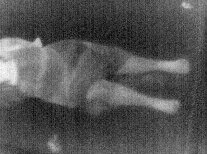
\includegraphics[scale=0.85]{TweedeExperiment_img0}
	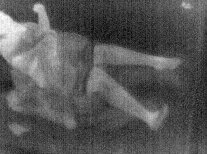
\includegraphics[scale=0.85]{TweedeExperiment_img4}
	\caption{Voorbeelden van opgeslagen afbeeldingen tijdens tweede experiment}
	\label{imgTEx1}
\end{figure}
Dit experiment is op twee verschillende manieren uitgevoerd. Dit omdat we niet tevreden waren met de resultaten die we de eerste keer verkregen. We bespreken eerst de eerste poging en vervolgens de tweede poging. 
\subsubsection{Eerste poging}
\label{ERefDUBEP}
\begin{figure}[h]
	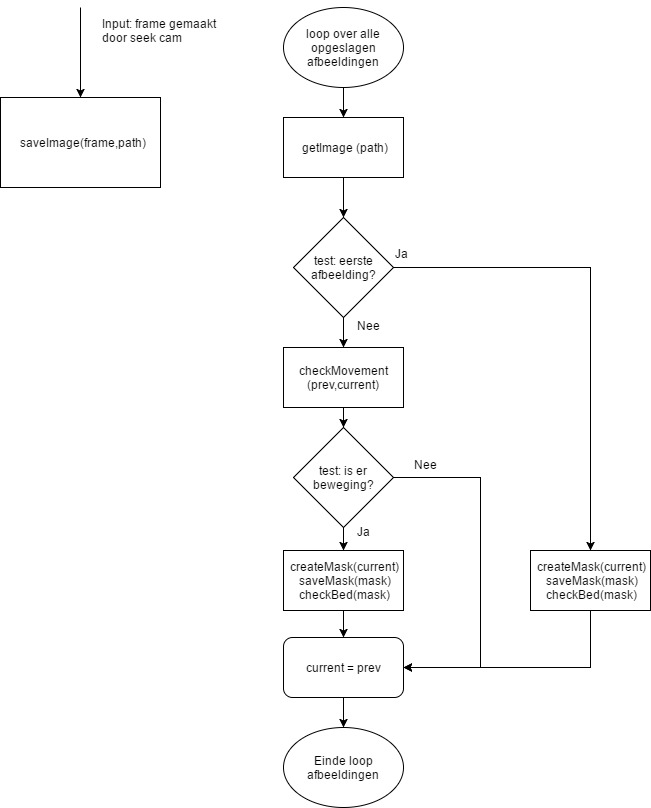
\includegraphics[scale=0.45]{FlowChart_DetectUitBed_EerstePoging}
	\caption{Flowchart eerste poging detectie uit bed stappen}
	\label{imgFCDUBEP}
\end{figure}
Om het idee achter dit experiment te verduidelijken voegen we een flowchart toe met daarin de gebruikt methodes om tot onze resultaten te komen, dit flowchart vidt u terug in figuur \ref{imgFCDUBEP}. We houden hier wel rekening met bewing om rekentijd de besparen. Maar we controleren nergens of de oppervlakken in het masker die het alarm gaan triggeren wel bewegende delen zijn of onderdelen van de achtergrond. De gebruikte methodes worden allemaal besproken in de sectie code \ref{mrefCod}

\subsubsection{Tweede poging}
\label{ERefDUBTP}
\begin{figure}[h]
	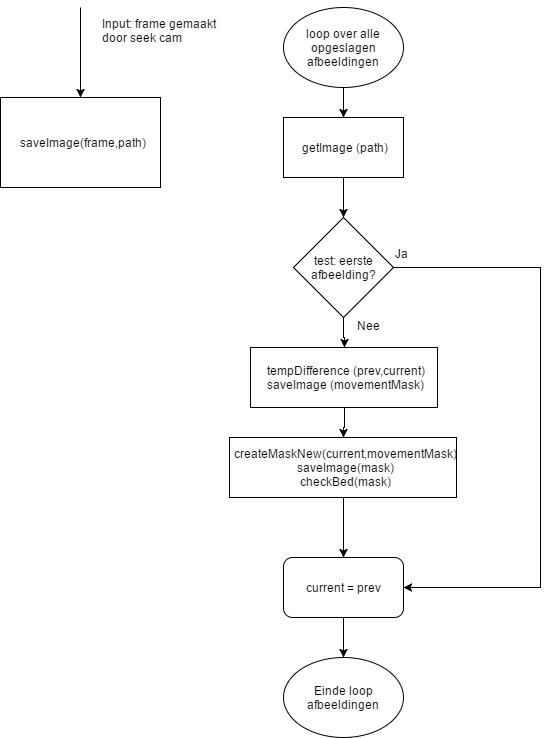
\includegraphics[scale=0.45]{FlowChart_DetectUitBed_TweedePoging}
	\caption{Flowchart tweede poging detectie uit bed stappen}
	\label{imgFCDUBTP}
\end{figure}
Nadat we onze conclusies hebben getrokken uit de eerste poging van ons experiment \ref{CRefDUBEP}, hebben we onze code aangepast. Het flowchart van deze aanpassingen vindt u in figuur \ref{imgFCDUBTP}. Het grootste verschil is dat we hier een temporeel verschil berekenen. Dit wordt opgeslagen als bewegingsmasker. Hierdoor gaan warme punten in de achtergrond, het alarm niet meer triggeren. De gebruikte methodes worden besproken in \ref{mrefCod}.

\subsection{Besluiten na de experimenten}
\label{ERefDBB}
In dit bespreken we de conclusies die we hebben getrokken uit het detecteren van het uit bed stappen. De conclusie over dit stukje wordt in twee delen gesplitst. Dit omdat de resultaten van de geruikte code in het eerste deel niet volstaat, daarna hebben we een paar aanpassingen in onze code gemaakt, de conclusies die we trekken na het toepassen van deze nieuwe code wordt als laatste besproken.

\subsubsection{Eerste poging}
Bij het bekijken van de resultaten van het tweede experiment, valt bij het maken van de maskers op dat er een lichtere vlek (rechtsbovenaan), ook mee gedetecteerd wordt, dit is echter geen deel van een persoon. De maskers ziet u in figuur \ref{imgCDUB}.
\begin{figure}[h]
	
\includegraphics[scale = 0.75]{MaskTweedeExperiment_img0}
	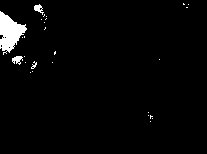
\includegraphics[scale = 0.75]{MaskTweedeExperiment_img4}
	\caption{Verkregen masker voor twee voorbeelden bij experiment twee}
	\label{imgCDUB}
\end{figure}
Hierdoor krijgen we steeds de melding dat de persoon uit het bed probeert te stappen langs de rechterzijde. Dit is natuurlijk een fout. Een mogelijke oplossing voor dit probleem is eerst detecteren welke pixels verandert zijn, daar is dus een beweging. Vervolgens kunnen we voor de bewogen pixels kijken welke warm genoeg zijn om tot de persoon te behoren. Zo kunnen we deze valse detecties vermijden. Hierdoor gaat de computer wel veel meer moeten rekenen.

\subsubsection{Tweede poging}
Nadat we eerst het temporeel verschil berekenen voor we het masker maken van de lichaamswarmte op de infraroodbeelden, kunnen we door gebruik te maken van de setSidesOfBed methode van de klasse Bed bepalen langs welke kant de persoon uit het bed probeerd te stappen. Als de persoon binnen de randen van het bed blijft wordt er None terug gegeven. Indien de randen van het bed wel wordt overschreven, wordt links of rechts (naargelang langs welke kant de rand wordt overschreven) afgedrukt op het scherm. Uit deze tweede poging van dit experiment kunnen we besluiten dat de detectie van langs welke zijde de persoon uit het bed stapt correct werkt. Het meten van de tijd dat een persoon weg blijft, is momenteel nog onmogelijk door de restwarmte die we nog zien in onze beelden. Een mogelijke oplossing hiervoor wordt in een volgend experiment aangeboden. 

\section{Experiment met live beelden}
\label{ERefELB}
De totale bespreking van het experiment op live beelden wordt uit gelegd in drie verschillende delen. We beginnen met te verklaren wat het doel \ref{ERefLBD} van dit experiment was, hierna bespreken we de opbouw en de uitwerking van het experiment \ref{ERefLBV}. Als laatste bespereken we de besluiten die we trekken uit dit experiment. 

\subsection{Doel van het experiment}
\label{ERefLBD}
Het doel van dit experiment is na te gaan of we de veranderingen in de beelden snel genoeg detecteren. We gaan dus testen of de detectie van langs welke zijde er aanstalten gemaakt worden om uit bed te stappen ook ogenblikkelijk gebeuren. 

\subsection{Uitwerking van het experiment}
\label{ERefLBV}
We  hebben ons systeem aangesloten op de camera en live beelden verwerkt. De proefopstelling is het zelfde gebleven als bij het vorige experiment \ref{ERefDUB}. Een schets hiervan ziet u in figuur \ref{imgTEx}. Tijdens dit experiment is er een persoon in het bed gaan liggen en heeft een paar keer gedaan als hij uit het bed wou stappen. Terwijl op het scherm in het oog werd gehouden of de computer de juiste detecties werden gemaakt.

\subsection{Besluiten na het experiment}
 Uit dit experiment kunnen we besluiten dat het systeem werkt. Vanaf er een arm of een been uit het bed wordt gestoken wordt er een melding gegenereerd met de juiste zijde. Het genereren van deze melding gebuerd vrijwel onmiddelijk. Kleding en deken vormt hier nog het grootste probleem. Als het lichaam bedekt is, wordt het door het masker niet gedetecteerd. Hierdoor zouden er evenementen gemist kunnen worden. Verder loopt het ook mis als er een persoon in het bed heeft gelegen en er uit stapt. De camera detecteerd dan de restwarmte an het bed en gaat doen alsof er wel nog een persoon in ligt. Zoals reeds eerder is aangehaald, wordt hiervoor in een volgende experiment een oplossing gezocht. 


\chapter{Algemeen besluit}
Het systeem detecteerd goed langs welke zijde er uit het bed gestapt wordt. Een mogelijk uitbereiding is de timer van hoelang een persoon uit bed is. Momenteel lukt dit nog niet door de restwarmte van het bed. Indien er ook wenst gewerkt te worden zonder de afbeeldingen op te slagen moet er ook nog aan de code gewerkt worden. De beelden die door de camera worden geleverd staan in een ander formaat als de beelden die ik verwerk, bijgevolg moeten er dan nog een paar kleine aanpassingen gebeuren. Verder kan er ook nog onderzoek gebruiken naar het gebruik van een night vision camera, om het probleem van de restwarmte te verkleinen. Verder kunnen ook andere cameras eens getest worden, de meeste mensen klagen over het klikgeluidje dat de camera maakt.

% Bibliografie: referenties. De items zitten in bibliografie.bib
%%%%%%%%%%%%%%%%%%%%%%%%%%%%%%%%%%%%%%%%%%%%%%%%%%%%%%%%%%%%%%%%%
% Indien je ook de niet geciteerde werken in je bibliografie wil opnemen, commentarieer dan onderstaande regel uit!
%\nocite{*}
\bibliographystyle{abbrv}
\bibliography{bibliografie}

% Eventueel enkele appendices
%%%%%%%%%%%%%%%%%%%%%%%%%%%%%%
\appendix
%\input{bijlage1}

% Bijlage met daarin het wetenschappelijk artikel
%%%%%%%%%%%%%%%%%%%%%%%%%%%%%%%%%%%%%%%%%%%%%%%%%%
%\chapter{Beschrijving van deze masterproef in de vorm van een wetenschappelijk artikel}
%\includepdf{artikel.pdf}

% Bijlage met daarin de poster
%%%%%%%%%%%%%%%%%%%%%%%%%%%%%%%
%\chapter{Poster}
%\includepdf{poster.pdf}


\includepdf{back_fiiw_denayer.pdf}
% 
\includepdf{back_fiiw_denayer_eng.pdf} % For the english version

\end{document}
